\documentclass[a4paper,cleardoubleempty,BCOR1cm, 11pt]{report}
% use to waste space:
% \documentclass[12pt,a4paper]{article}

% if you have this style and like it.
%\documentclass{acmsiggraph}
%\documentclass[review]{acmsiggraph}      % review
%\documentclass[widereview]{acmsiggraph}  % wide-spaced review
%\documentclass[preprint]{acmsiggraph}    % preprint

% define a \comment{this is a comment which can have linebreaks in it}
\newcommand{\comment}[1]{}
% \newcommand{\todo}[1]{\marginpar{\bf{#1}}}
\newcommand{\todo}[1]{{\color{red}\bf{TODO: #1}}}
\usepackage{booktabs}
\usepackage{mathptmx}
\usepackage[pdftex]{graphicx}
\usepackage[pdftex]{color}
\definecolor{rot}{RGB}{165,30,55} %rote Farbe
\definecolor{lila}{RGB}{90,0,91} %rote Farbe
\definecolor{schwarz}{RGB}{0,0,0}
\graphicspath{{./images/}}
\usepackage{parskip}
\usepackage{amsmath}
\usepackage{dsfont}
\usepackage{pxfonts}
\usepackage{natbib}
\usepackage{setspace}

\usepackage[paper=a4paper,left=25mm,right=35mm,top=25mm,bottom=20mm, includehead, includefoot, twoside]{geometry}
\usepackage[T1]{fontenc}
\usepackage{textcomp}

% comment these two lines out if you don't want minion/myriad fonts.
% \usepackage[minionint,mathlf]{MinionPro}
% \renewcommand{\sfdefault}{Myriad-LF}
%\usepackage{Myriad}

% no page number on float pages, fixes problems with overlarge diagrams.
\usepackage{fancyhdr}
\pagestyle{fancy}
%\lhead{}
%\chead{}
%\rhead{}
%\lfoot{}
\fancyhf{}
\fancyhead[EL]{\nouppercase{\leftmark}}
\fancyhead[OR]{\nouppercase{\rightmark}}
\cfoot{}
%\fancyfoot[EL]{\iffloatpage{}{\thepage}}
%\fancyfoot[OR]{\iffloatpage{}{\thepage}}
\fancyfoot[EL]{\thepage}
\fancyfoot[OR]{\thepage}
\renewcommand{\headrulewidth}{0pt}
\renewcommand{\footrulewidth}{0pt}

%\usepackage{natbib}		% textual referencing
%\usepackage[numbers,super]{natbib}	% nice superscripts
%\bibliographystyle{chicago}	% shitty
%\bibliographystyle{alpha}	% abbr names and year in \cite
%\bibliographystyle{agsm}	% australian, need natbib
%\bibliographystyle{kluwer}	% need natbib
\bibliographystyle{apalike}	% lengthly
%\bibliographystyle{abbrv}	% minimal?

% use for german line breaking:
%\usepackage[ngerman]{babel}
\usepackage[T1]{fontenc}
\usepackage[utf8x]{inputenc}

% avoid us-style text color destruction:
\frenchspacing
\usepackage{microtype}

% have a nice framebox with border directly around the image:
\fboxsep 0pt
\newcommand{\fimg}[2]{\fbox{\includegraphics[width=#1]{#2}}}

\usepackage{theorem}
\theorembodyfont{\upshape}
\newtheorem{definition}{Definition}

\usepackage{listings}
\lstset{numbers=left, numberstyle=\tiny, basicstyle=\tiny, language=Python}
%\usepackage[boxruled]{algorithm2e}
\usepackage{algorithm,algorithmic}% http://ctan.org/pkg/algorithms
%\usepackage{hyperref}
\usepackage{url}
\usepackage{subfig}

\def\code#1{{\tt{#1}}}



\begin{document}
\vspace*{10ex}
Bachelorarbeit

{\huge\bf\textsf{Uncertainty in Recurrent Decision Tree Classifiers}}

\vspace*{30ex}

Eberhard Karls Universität Tübingen\\
Mathematisch-Naturwissenschaftliche Fakultät\\
Wilhelm-Schickard-Institut für Informatik\\
Explainable Machine Learning\\
Stefan Wezel,~ \verb+stefan.wezel@student.uni-tuebingen.de+,~ 2020

\vspace*{5ex}

\begin{tabular}{@{}l@{\hspace{2em}}l}
	Bearbeitungszeitraum:& von-bis \vspace*{5ex} \\
	Betreuer/Gutachter:& Prof. Dr. Zeynep Akata, Universität Tübingen\\
	Betreuer:& Stephan Alaniz, Max Planck Institut für Informatik
\end{tabular}

\thispagestyle{empty}
%\newpage
	


%\begin{tabular}{lr}
%
\includegraphics[width=0.5\linewidth]{logo_sw} % logo bw
 
\includegraphics[width=0.5\linewidth]{UT_WBMW_Rot_4C} % logo red
 & \hspace{0.2\linewidth}
 \parbox{0.5\linewidth}{
   \large\bf\textsf{\color{schwarz}{Mathematisch-\\Naturwissenschaftliche\\Fakultät\\\\}}
   \hspace{-.144cm}\normalsize\textsf{\color{lila}{Explainable Machine Learning}}
   \vspace{0.6cm}
 }
\end{tabular}

\vspace*{10ex}
Bachelorarbeit

{\huge\bf\textsf{Uncertainty in Recurrent Decision Tree Classifiers}}

\vspace*{30ex}

Eberhard Karls Universität Tübingen\\
Mathematisch-Naturwissenschaftliche Fakultät\\
Wilhelm-Schickard-Institut für Informatik\\
Explainable Machine Learning\\
Stefan Wezel,~ \verb+stefan.wezel@student.uni-tuebingen.de+,~ 2020

\vspace*{5ex}

\begin{tabular}{@{}l@{\hspace{2em}}l}
  Bearbeitungszeitraum:& von-bis \vspace*{5ex} \\
  Betreuer/Gutachter:& Prof. Dr. Zeynep Akata, Universität Tübingen\\
  Betreuer:& Stephan Alaniz, Max Planck Institut für Informatik
\end{tabular}

\thispagestyle{empty}
\newpage

\chapter*{Selbstst\"andigkeitserkl\"arung}
Hiermit versichere ich, dass ich die vorliegende Bachelorarbeit selbst\"andig und
nur mit den angegebenen Hilfsmitteln angefertigt habe und dass alle Stellen,
die dem Wortlaut oder dem Sinne nach anderen Werken entnommen sind,
durch Angaben von Quellen als Entlehnung kenntlich gemacht worden sind.
Diese Bachelorarbeit wurde in gleicher oder \"ahnlicher Form in keinem anderen
Studiengang als Pr\"ufungsleistung vorgelegt.

\vspace*{8ex}
\hrule
\vspace*{2ex}
Stefan Wezel (Matrikelnummer 4080589), \today


\chapter*{Abstract}
Recurrent Decision Tree Classifiers have proven to be capable of providing explanations of their classification while yielding state of the art results in prediction accuracy on several image classification tasks. However, we show that they may utilize features that they are highly uncertain about. We hypothesize that when using uncertainty information, the RDTC can provide more faithful explanations and become more applicable in real-life scenarios.
Based on RDTC, we propose two models that utilize uncertainty information. We either enhance the vocabulary of RDTC with an uncertainty token, allowing for a ternary decision tree, or, we restrict the RDTC from using uncertain attributes.
We investigate how uncertainty information can be used in generating interpretable model outputs and how it affects the models performance on several benchmark tasks.





\tableofcontents

%% braucht kein Mensch ...
%\listoffigures
%\listoftables


\chapter{Introduction}
% Motivation for explainabiltiy and uncertainty
The recent surge in popularity of machine learning methods has made the fields ambivalent nature obvious. Public opinion is split between hype and mistrust. 
Systems, using machine learning have failed at seemingly simple tasks \cite{kelion2018ces}, displayed racist and sexist behavior \cite{guynn2015google, schlesinger2018let, zou2018ai} and even caused fatalities \cite{yadron2016tesla}.
Such cases, where an artificial intelligence has made severe mistakes are funny at best and outright dangerous at worst. Most importantly, they have made it clear that, despite being deployed more frequently than ever before, machine learning has yet to prove itself \cite{schlesinger2018let, dikmen2016autonomous, zou2018ai}.
These cases show that methods that allow introspection and behave faithfully are more important than ever.\\
Addressing such issues, \citet{alaniz2019explainable} propose a model that can reliable justify its classification through stating utilized features in a decision tree. Here, we build on this method. We extend the model, so that it is aware of and able to express its own uncertainties. We hypothesize that such a model may be perceived by a user as more trustful than a model that does not.\\
% more motivation on uncertainty
We, as humans have developed an intuition how do make decisions under uncertainty \cite{bland2012different} and are able to operate in a domain of limited and noisy data. Moreover, uncertainty is an important measure in science that allows to express how well something is known or can be known. Scientists from fields like medicine, physics or meteorology rely on uncertainty information for making and communicating decisions or predictions. Outside the scientific world, uncertainty information is important in finance or law among others \cite{liu2013toward, d1983legal}.\\
Uncertainty information is valuable. Especially in real-world scenarios, where we might encounter only limited, or noisy data to learn from. Where predictions, far into the future are required. Or, where decisions with high consequences have to be made. 
As machine learning becomes more prevalent in our everyday lives, in science, finance, or law, the need for methods, utilizing uncertainty becomes more evident.\\
% overconfidence of softmax and uncertainty
Unfortunately, the output of most neural network architectures does not contain uncertainty information. For example, in classification, typical architectures use a softmax layer, to turn model outputs into a probability density function \cite{nwankpa2018activation} over classes. Since it is a probability distribution, the softmax output is often misinterpreted as a measure of how certain a model is regarding each class \cite{sensoy2018evidential}. However, this distribution only arises from each value relative to every other value and is a point estimate, turned into a distribution. The point estimate cannot carry any uncertainty information and the softmax certainly does not add such. This allows a softmax class probability to be overconfident for a highly uncertain class \cite{gal2016dropout}.
% Key contributions
Our key contributions are to propose a model, that allows to (1) study the effect of (epistemic) uncertainty for attribute based recurrent decision tree classifier and actively uses and expresses uncertainty information. We (2) test the proposed models performance on popular datasets and compare it to different state-of-the-art methods. We investigate uncertainties in the model and data and evaluate its affect on performance. \\
% Example applications
Such a model may be applied in settings, where a high confidence classification for out-of-domain examples may have severe consequences. For example in medical settings, in law or in autonomous driving. There, in cases of high uncertainty, a human could be notified and consulted, preventing the model from making a (potentially wrong) high-risk decision. The model would still provide a decision tree as explanation, which could be utilized by a human user to make a final decision.




\chapter{Related Work}
Building on, often centuries old, mathematical foundations, and on more recent psychological and neurobiological insights, machine learning has evolved throughout the last decades and a vast corpus of literature has emerged from this development. Here we will briefly go over some historic aspects, introduce important concepts and give an overview of the current state of explainable methods and uncertainty in machine learning. 


\section{Neural Networks}
Artificial neural networks (ANNs) have become an integral part in the lifes of many. Inspired by the cognitive processes of the mammalian brain, several architectures and learning algorithms have been proposed.

\subsection{Historical Context}
The idea of artificial intelligence (AI) is dating back to antiquity and was debated in various domains ranging from chemistry \cite{o1994alchemical} to philosophy and mathematics \cite{leibnizdissertatio}. A watershed moment in its development is marked by \citet{mcculloch1943logical}, who modeled a neuron in an approach that unified findings from neurophysiology and mathematics. Later, \citet{hebb19680} proposed a theory of how the strengthening and weakening of connections between neurons encodes gained knowledge(?).  This idea was also applied in the perceptron \cite{rosenblatt1960perceptron} which could learn distinguish linearly separable classes. 
\citet{marvin1969perceptrons} showed that the perceptron was more useful when connecting many and using a middle layer in a so called multilayer perceptron (MLP). If this hidden layer has a non-linear activation function it could learn to classify not linearly separable data. This idea of many simple but connected units remains a key principle in ANNs.
However, simulating the behavior of neural networks requires many computations and the sequential nature of hardware available at the time prohibited connectionist ideas to be applied in practice.\\
Over the decades, ANNs have risen and fallen in popularity among AI researchers. Different architectures and learning algorithms have been proposed but many failed to establish. Important milestones were \citet{rumelhart1986learning}, who extended learning rules to MLPs in the backpropagation algorithm, the Long short-term memory by \citet{hochreiter1997long}, and the convolutional neural net (CNN), proposed by \citet{lecun1995convolutional} which allowed to classify handwritten digits.\\
However, these methods still failed to establish far beyond the realm of research. The development of graphics processing units (GPUs) and the availability of large scale datasets have caused this to change in the 2010s where for some tasks ANNs have exceeded human performance \cite{ILSVRC15}.


\subsection{Multilayer Perceptron}\label{sec:MLP}
The MLP is a rather simple architecture. It consists of an input layer, an arbitrary number of hidden layers and an output layer. Each neuron is typically connected to each neuron in the next layer. Thus each neuron gets the weighted output from the last layer's neurons as input. Non-linear activation functions allow the network to learn not linearly separable problems. 


\begin{figure}
	\centering
	\begin{minipage}[t]{0.45\textwidth}
		\centering
		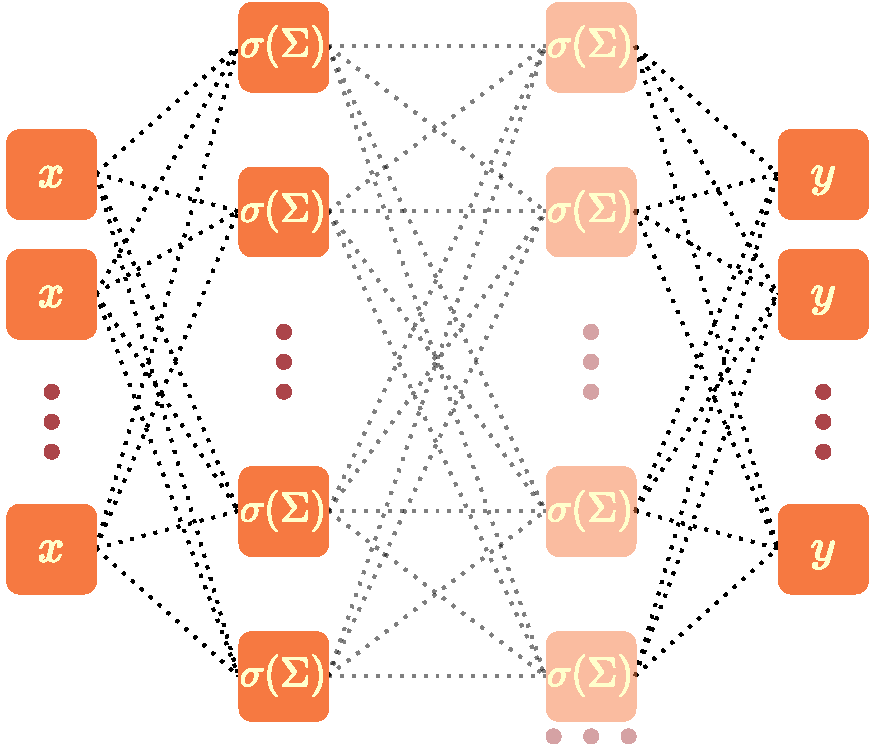
\includegraphics[width=0.8\textwidth,height=0.21\textheight]{images/mlp.pdf} 
		\caption{A MLP can consists of an input layer, an arbitrary number of hidden layers, and an output layer.}
	\end{minipage}\hfill
	\begin{minipage}[t]{0.45\textwidth}
		\centering
		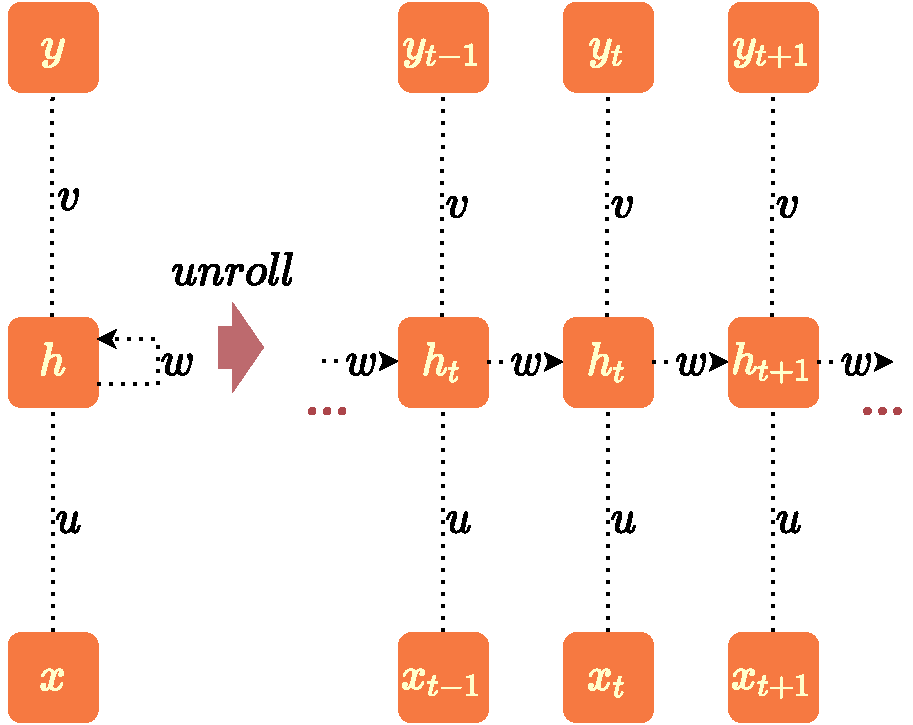
\includegraphics[width=0.9\textwidth,height=0.20\textheight]{images/rnn.pdf}
		\caption{The recurrent neural network takes in an input for every time step as well as its own hidden state.}
		\label{fig:rnn}
	\end{minipage}
\end{figure}




\subsection{Recurrent Neural Networks}
Many types of data don't provide samples of fixed length. This is the case for most language or time series data among others. A MLP, however, is incapable of processing such samples due to its fixed amount of input neurons. To alleviate this, recurrent neural networks (RNNs) use the output of their neurons as an input after being multiplied with a weight matrix. Many concepts of RNNs exist \cite{Grossberg:2013}. Here we will have a closer look at a very simple example, depicted in Figure \ref{fig:rnn}.
The  RNN takes in an input $in_t$ which is transformed by weight matrix $u$ and added to the hidden state of the last time step times weight matrix $w$. This forms the hidden state of the current time step. To obtain an output at a given time step, the hidden state is multiplied with weight matrix $v$. The update rules can be stated as:
\begin{align}
	h_t &= f_{act}(u \circ in_t + w \circ h_{t-1})\\
	out_t &=f_{act}(v \circ h_t)
\end{align}
A RNN can be trained by the Backpropagation through time algorithm (BPTT). \citet{werbos1990backpropagation} propose to unfold a RNN for each time step or element of the input. This unfolding makes it equivalent to a feed-forward ANN (such as the MLP introduced in Subsection \ref{sec:MLP}) and weights can be adjusted according to the gradients.


\subsection{Convolutional Neural Networks}
CNNs have proven to be useful tool for various image related tasks. They are a type of feed-forward network with the underlying concept of learning filters that correspond to features in the data. Typically this is done over multiple layers with the intention of learning to recognize low level concepts such as edges in layers close to the input layer and high level concepts in layers further away from the input. In practice, after convolutions and non-linearities are applied, the results are usually subsampled, using a pooling operation to reduce the amount of necessary parameters.

\begin{figure}
	\centering
		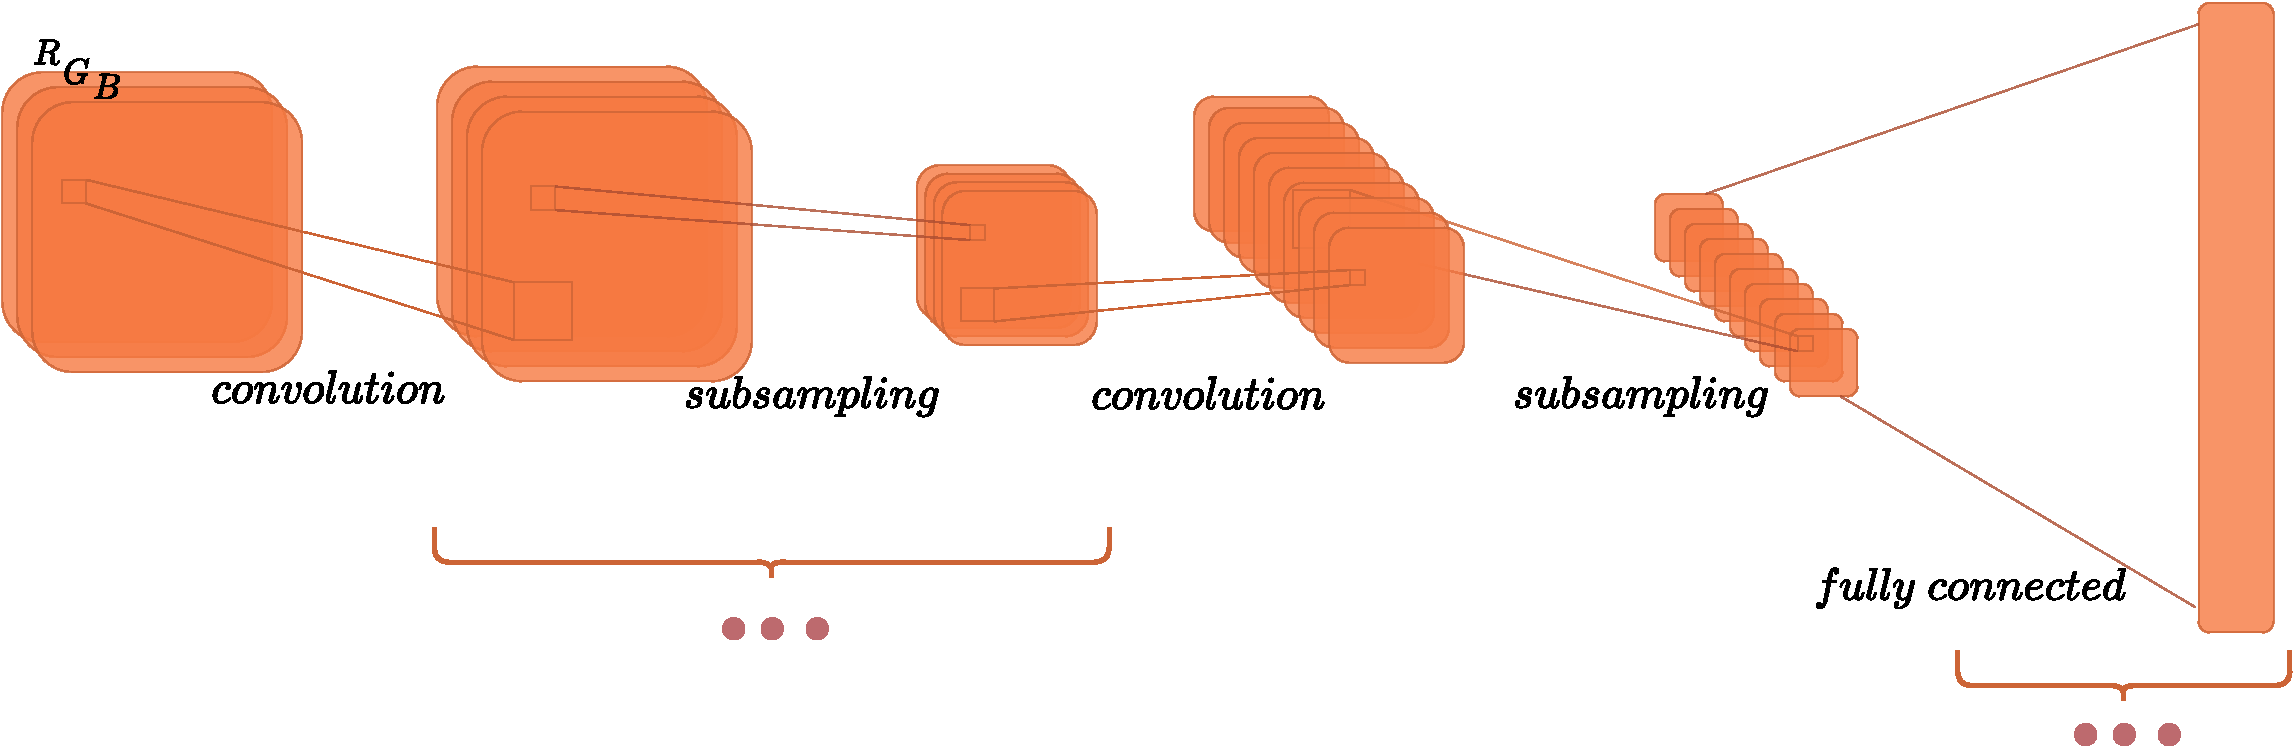
\includegraphics[width=0.9\textwidth]{images/convnet.pdf} 
		\caption{A CNN with two convolutional and subsampling layers which can be repeated arbitrary times.}
		\label{fig:convnet}
\end{figure}


\section{Explainable Machine Learning}
While interpretable models exist in machine learning, they are often outperformed by modern ANNs with a large number of parameters, on a variety of tasks \cite{gunning2019xai, guo2020explainable, sarkar2016accuracy, puiutta2020explainable}. Understanding the processes inside a model with a large number of parameters is not trivial. Thus, various approaches have been developed to understand a models decision process for given data. Such methods, that are interpretable or can explain their decisions are inevitable for safety critical applications. They allow a human user to understand how a model came to a certain output and allow for a faithful human-AI interaction to emerge.


\subsection{Decision Trees}
Decisions trees provide an inherently interpretable model. Given data with features $a_1, ..., a_n$ a decision tree iteratively splits data according to conditions for each attribute. Splits occur for each attribute $a_i$ where samples from data are either above or below a given threshold for their values of $a_i$. Optimal splits can be found by learning algorithms or by expert knowledge. Nodes represent the resulting splits and edges represent the corresponding answer.
Decision trees are a frequently used tool in data mining \cite{wu2008top}. Popular algorithms to generate decision trees from data include Iterative Dichotomiser 3 and C4.5, both suggested by Quinlan \cite{quinlan1986induction,quinlan2014c4}.
Another popular algorithm is Classification and Regression Trees, introduced by \citet{breiman1984classification}. The key concept behind these algorithms is to create splits that maximize information gain for each available attribute.\\
In order to reduce size and increase interpretability of generated trees, pruning can be applied \cite{mingers1989empirical}. Pruning can also reduce the risk of overfitting (\cite{kearns1998fast}).

\begin{figure}
	\centering
	\begin{minipage}[t]{0.45\textwidth}
		\centering
		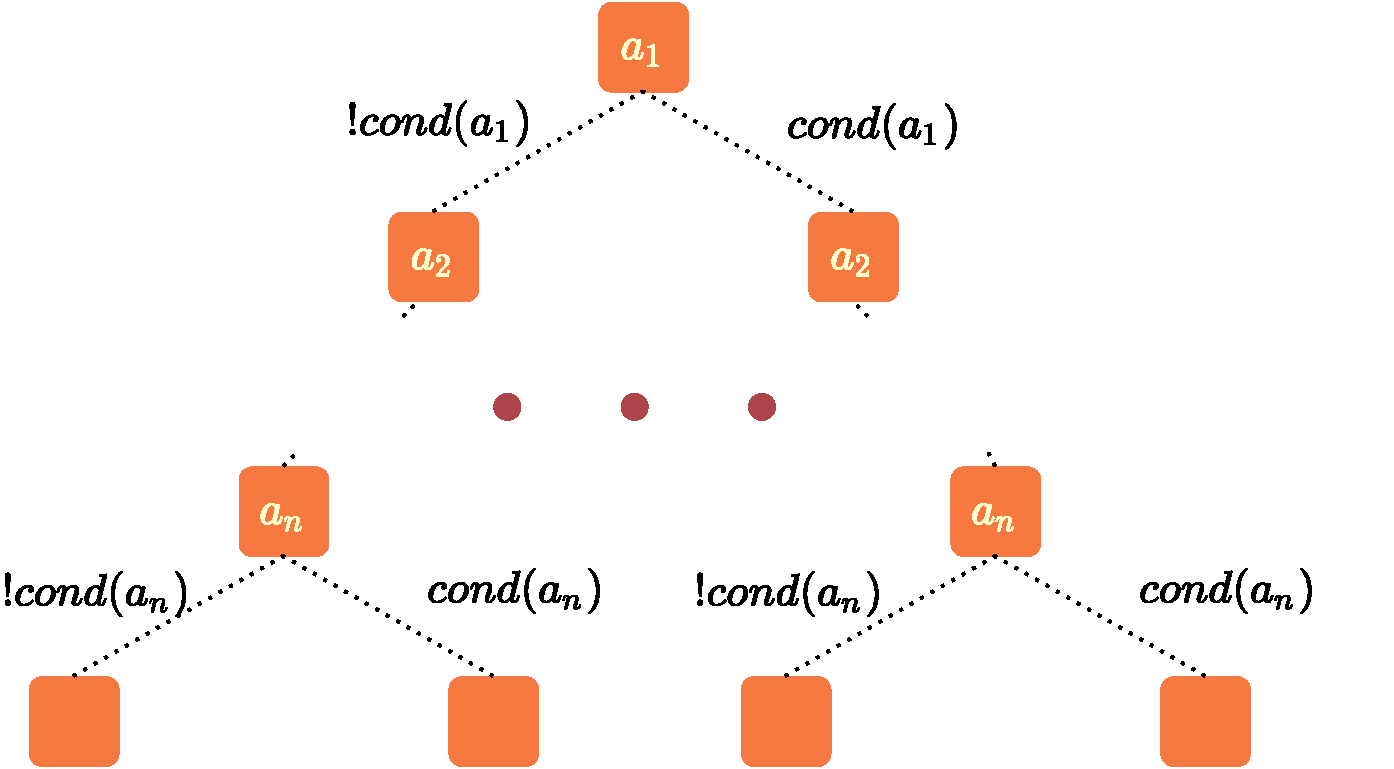
\includegraphics[width=0.9\textwidth,height=0.16\textheight]{images/decisiontree.pdf} 
		\caption{A decision tree splits data according to values of attributes.}
		\label{fig:decision_tree}
	\end{minipage}\hfill
	\begin{minipage}[t]{0.45\textwidth}
		\centering
		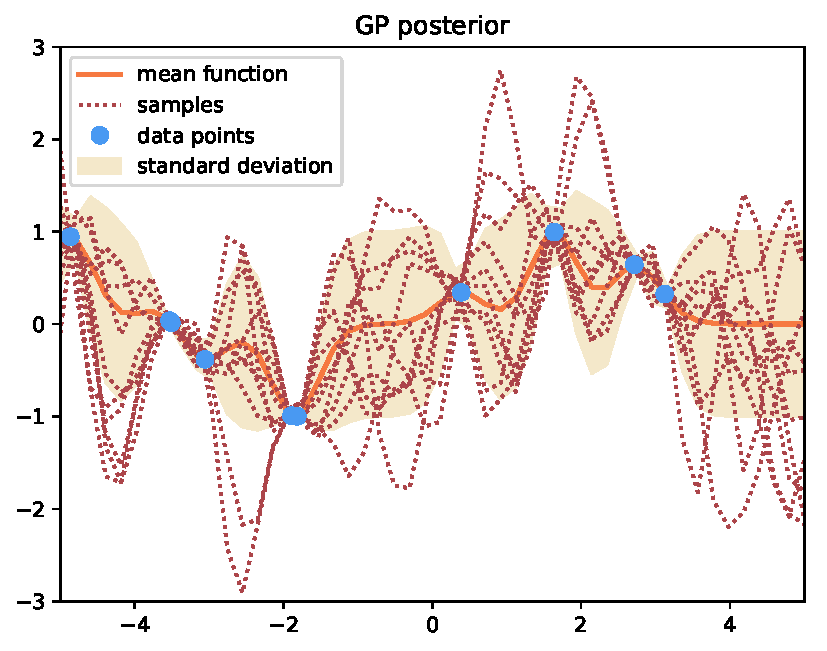
\includegraphics[width=0.9\textwidth,height=0.16\textheight]{images/post.pdf}
		\caption{A Gaussian process is a distribution over the space of functions that describe data (blue).}
	\end{minipage}
\end{figure}



\subsection{Leveraging Attributes}
While decision trees are suitable for tabular data, applying them on image data is not trivial. Images are parameterized by pixels rather than attributes, so attributes have to be provided as side information. Ideally, those attributes should correspond to features that characterize classes found in the image data. Therefore, a popular way of acquiring side information is by humans label the data according to characteristics suggested by domain experts. \citet{WahCUB_200_2011} let users label different kind of bird species according to attributes and collect them in the CUB dataset. Another dataset containing attributes as side information is proposed by \citet{8413121}.\\
Attributes can be used to create an interpretable output of a neural network. \citet{akata2013label} propose to learn a linear mapping between feature representations learned by a neural network and learned attribute representations.
In other areas, attributes are used as well. \citet{kulkarni2013babytalk} and \citet{ordonez2011im2text} use attributes for image captioning. \citet{lampert2009learning} and \citet{palatucci2009zero} use attributes for zero-shot learning.


\subsection{Multi-agent Communication}
Communication between different agents is a popular technique in reinforcement learning \cite{havrylov2017emergence, lazaridou2018emergence, cao2018emergent, jiang2018learning, das2019tarmac}. \citet{foerster2016learning} propose to let one agent send messages containing categorical symbols which can be used by a second agent to solve a problem. Multi-agent communication has also been used for the purpose of creating interpretable outputs by \citet{rodriguez2019modeling} who take in account that different agents may have differing understanding of concepts. Communication between two agents is also the basis for learning in the RDTC, proposed by \citet{alaniz2019explainable}, which our work builds on.

\section{Uncertainty}
Uncertainty is an important factor in human decision making. Modeling uncertainty in machine learning methods is useful for ensuring responsible decision making of algorithms and allows a user to build trust in these models. Uncertainty can arise from data. This is called aleatoric uncertainty. It compromises all kinds of noise inherent to the data. If this noise is static (i.e. limited precision of a sensor) it is call homoscedastic uncertainty. If noise is not static (i.e. occlusions in an image) the uncertainty is called heteroscedastic uncertainty.\\
On the other hand, a model can also be uncertain about its own parameters. This uncertainty is called epistemic uncertainty and is high if a model has seen few data. By giving it more data, it can be reduced. Those two kinds of uncertainty are displayed for a computer vision task in Figure \ref{fig:uncertainty_example}.
% image that shows the heteroscedastic and epistemic uncertainty
\begin{figure}
	\centering
	\includegraphics[width=0.9\textwidth]{images/uncertainty_example.png} 
	\caption{Areas with high aleatoric uncertainty are marked red. These are mostly due to occlusions in the image. The area in purple is due to high epistemic uncertainty, since the model has never seen a boat before. It misclassifies it as a car but is uncertain about this classification}
	\label{fig:uncertainty_example}
\end{figure}

\subsection{Bayesian Inference}
Applying Bayes' theorem to update prior beliefs as more data becomes available is called Bayesian inference \cite{box2011bayesian}. Bayes' theorem was introduced by \citet{bayes1763lii} and is stated as
\begin{align*}
	p(a|b) = \frac{p(b|a) \cdot p(a)}{p(b)}.
\end{align*}
Intuitively put, it computes the posterior conditional probability of a random variable $a$ given, the likelihood of $b$ being true, given $a$ is true: $p(b|a)$, a prior believe $p(a)$ and a marginalization term $p(b)$. Methods of Bayesian inference are popular in different fields of science, such as neurology, psychology, medicine, epidemiology, geography and machine learning \cite{friston2002classical,wagenmakers2018bayesian,koch2006bayesian,parmigiani2002modeling,didelot2014bayesian,ghahramani2015probabilistic}. They can be used to incorporate prior knowledge, multiple sources of evidence, or, in general, construct large joint probability density functions \cite{Spiegelhalter:2009}.




\subsection{Variational Inference}\label{sec:vi}
Methods of variational inference are used when intractable integrals are encountered in Bayesian inference \cite{jordan1999introduction}. Suppose, we want to find the predictive posterior $p(y^*|x^*, X,Y)$ for some datapoint $x^*$, we need to compute
\begin{align*}
p(y^*|x^*, X,Y) = \int p(y^*|x^*, w)p(w|X,Y)dw.
\end{align*}
The true posterior over model parameters, given data $p(w|X,Y)$ is not trivial to find an is often intractable in practice. Therefore an approximate distribution $q_{\theta}(w)$, with optimizable parameters $\theta$ is used. Ideally, $q_{\theta}(w)$ should be similar to the true posterior. Thus, we minimize the KL-divergence between the approximate distribution and the true posterior.
\begin{align*}
KL(q_{\theta}(w)|p(w|X,Y)).
\end{align*}
Given an approximate distribution, the predictive posterior can be written as
\begin{align*}
p(y^*|x^*) \approx \int p(y^*|x^*, w)q_{\theta}(w)dw.
\end{align*}
In order to find the variational distribution $q_{\theta}^*(w)$ with the optimal set of parameters, we have the objective
\begin{align*}
\mathcal{L}_{VI} := \int q_{\theta}(w) log\;p(Y|X, w)dw - KL(q_{\theta}(w)|p(w))
\end{align*}
that is optimized in respect to to parameters $\theta$. Here, $p(w)$ is a prior that is often assumed to be a standard Gaussian. According to \citet{bishop2006pattern}, maximizing the log evidence lower bound is equivalent to minimizing the KL-divergence but does not require having access to the true posterior $p(w)$. This effectively leaves us with an optimiziation task where we need to compute derivatives instead of integrals. This, in turn, allows us to apply powerful automatic differentiation tools, such as deep learning frameworks.



\subsection{Gaussian Processes}\label{sec:gp}
 %TODO citations
Gaussian processes are a powerful, generative model that can be applied to a variety of machine learning tasks \cite{mackay1998introduction}. They build on the notion that data can be described by (possibly infinitely) many functions. Gaussian processes (GPs) assign probabilities to functions that describe given data. Starting with a prior distribution over functions a GP returns a posterior over the space of functions, given new data. Of course, distributions over functions are somewhat hard to define. Therefore, we will view a function $f(x)$ as a vector where the $x$ denotes the index that will retrieve the function value at this point. Now, a GP is a joint normal distribution over the points of this vector, defined by a mean function $\mu(x)$ and a covariance function $\Sigma(x)$ with $\Sigma(x) = \Sigma_{ij} = k(x_i,x_j)$. The kernel function $k$ has to return a positive definite matrix and should return a high output for similar $x_i$ and $x_j$.\\
GPs thus view each $x_i$ as a random variable, that is dependent on all other $x_j\neq x_i$.\\
To perform inference in a GP, one simply takes the conditional probability density distribution (PDF) of a given $x_i$ conditioned on all other $x_j\neq x_i$. Since Gaussian distributions are closed under conditioning, the resulting PDF is Gaussian as well.\\
To retrieve a meaningful posterior from a GP, it has to be trained in a supervised fashion. We will describe the necessary steps in pseodocode.

\begin{algorithm}[ht]
\setlength{\leftskip}{4mm}
-create a prior-\\
$x_{test}$= $\lbrace x_n \rbrace$\\
$K_{prior}$ = kernel($x_{test}$, $x_{test}$, $w$)\\
$L_{prior}$ = cholesky\_decomposition($K_{prior}$)\\ % maybe square root instead of cholesky
$f_{prior}$ = $L_{prior} \cdot \mathcal{N}(dim=(n, num\_samples);0,1)$

-take new data into account and compute new posterior-\\
$x_{train}$, $y_{train}$ = training data\\
$K$ = kernel($x$, $x$, $w$)\\
$L$ = cholesky\_decomposition($K$)\\
$K_s$ = kernel($x_{train}$, $x_{test}$, $w$)\\
$L_k$ = solve($L$, $K_s$)\\
$\mu$ = $L_k^T \cdot$ solve($L, y_{train}$)\\

-draw samples from posterior-\\
$L$ = cholesky\_decomposition($K_{ss}$ - $L_k^T \cdot L_k$)\\
$f_{posterior}$ = $\mu$ + $L \cdot \mathcal{N}(dim=(n, num\_samples);0,1)$\\
- prediction at test point $x_i$ is now the sample's value at position $i$
\end{algorithm}
%TODO pseudocode




\subsection{Modeling Uncertainty in Neural Networks} %TODO maybe more motivation (with example)
%Alternative title: Dropout Variational Inference
Deep neural networks (DNNs) are applied in safety critical processes where information about a model's uncertainty is of crucial importance \cite{najafabadi2015deep}, \cite{krzywinski2013importance}. Standard DNN's however do not yield uncertainty information. Bayesian neural networks (BNNs) are an architecture that can model uncertainty reliably \cite{mullachery2018bayesian}. However, they require modeling a probability density function over each parameter which causes a high computational cost. A method using variance arising from dropout has been proposed by \citet{gal2016dropout} who proofed dropout in neural networks is equal to Monte-Carlo integration in GPs and thus can be used to model epistemic uncertainty.\\
%TODO proof here?



With a GP, we want to find a posterior distribution over function that explain given data. We can view a finite model like a neural network as an approximation to a GP \cite{damianou2013deep}. Thus, by optimizing a model, we minimize the Kullbach-Leibler (KL) divergence between our finite model and the corresponding GP \cite{gal2016dropout}. In practice, however, the GP's posterior often requires computing intractable integrals. To alleviate this, methods of variational inference, such as Monte-Carlo integration are applied. Monte-Carlo integration in a GP corresponds to averaging forward passes in a dropout neural net. According to \citet{gal2016dropout}, the resulting variance can be views as the model's uncertainty.
\\
Additionally, \citet{kendall2017uncertainties} propose to combine aleatoric and epistemic uncertainty in a unified approach. For classification tasks, this has been simplified by \citet{kwon2020uncertainty}.







\chapter{Uncertain RDTC} % aka Methods aka Architecture
The Recurrent decision tree model, proposed by \citet{alaniz2019explainable}, consists of two communication agents. Their common goal is to solve a classification task through communication. The Recurrent Decision Tree (RDT) agent has no direct access to data and can only ask question regarding the absence, presence or uncertainty of attributes. Given answers by the Attribute-based Learner (AbL) agent it can then store the answers thus incrementally building a decision tree that is used for the final classification. The learned decision three allows introspection.\\
Based on their work, we propose a model, where the AbL is able to express its uncertainty for given attributes. We use this uncertainty information by either preventing the RDT from using uncertain attributes or by allowing the AbL to answer with 'I don't know' additionally to the options 'Yes' or 'No'\footnote{We provide a Pytorch implementation of our model at \url{github.com/wastedsummer/urdtc}}. 



\begin{figure}
	\centering
	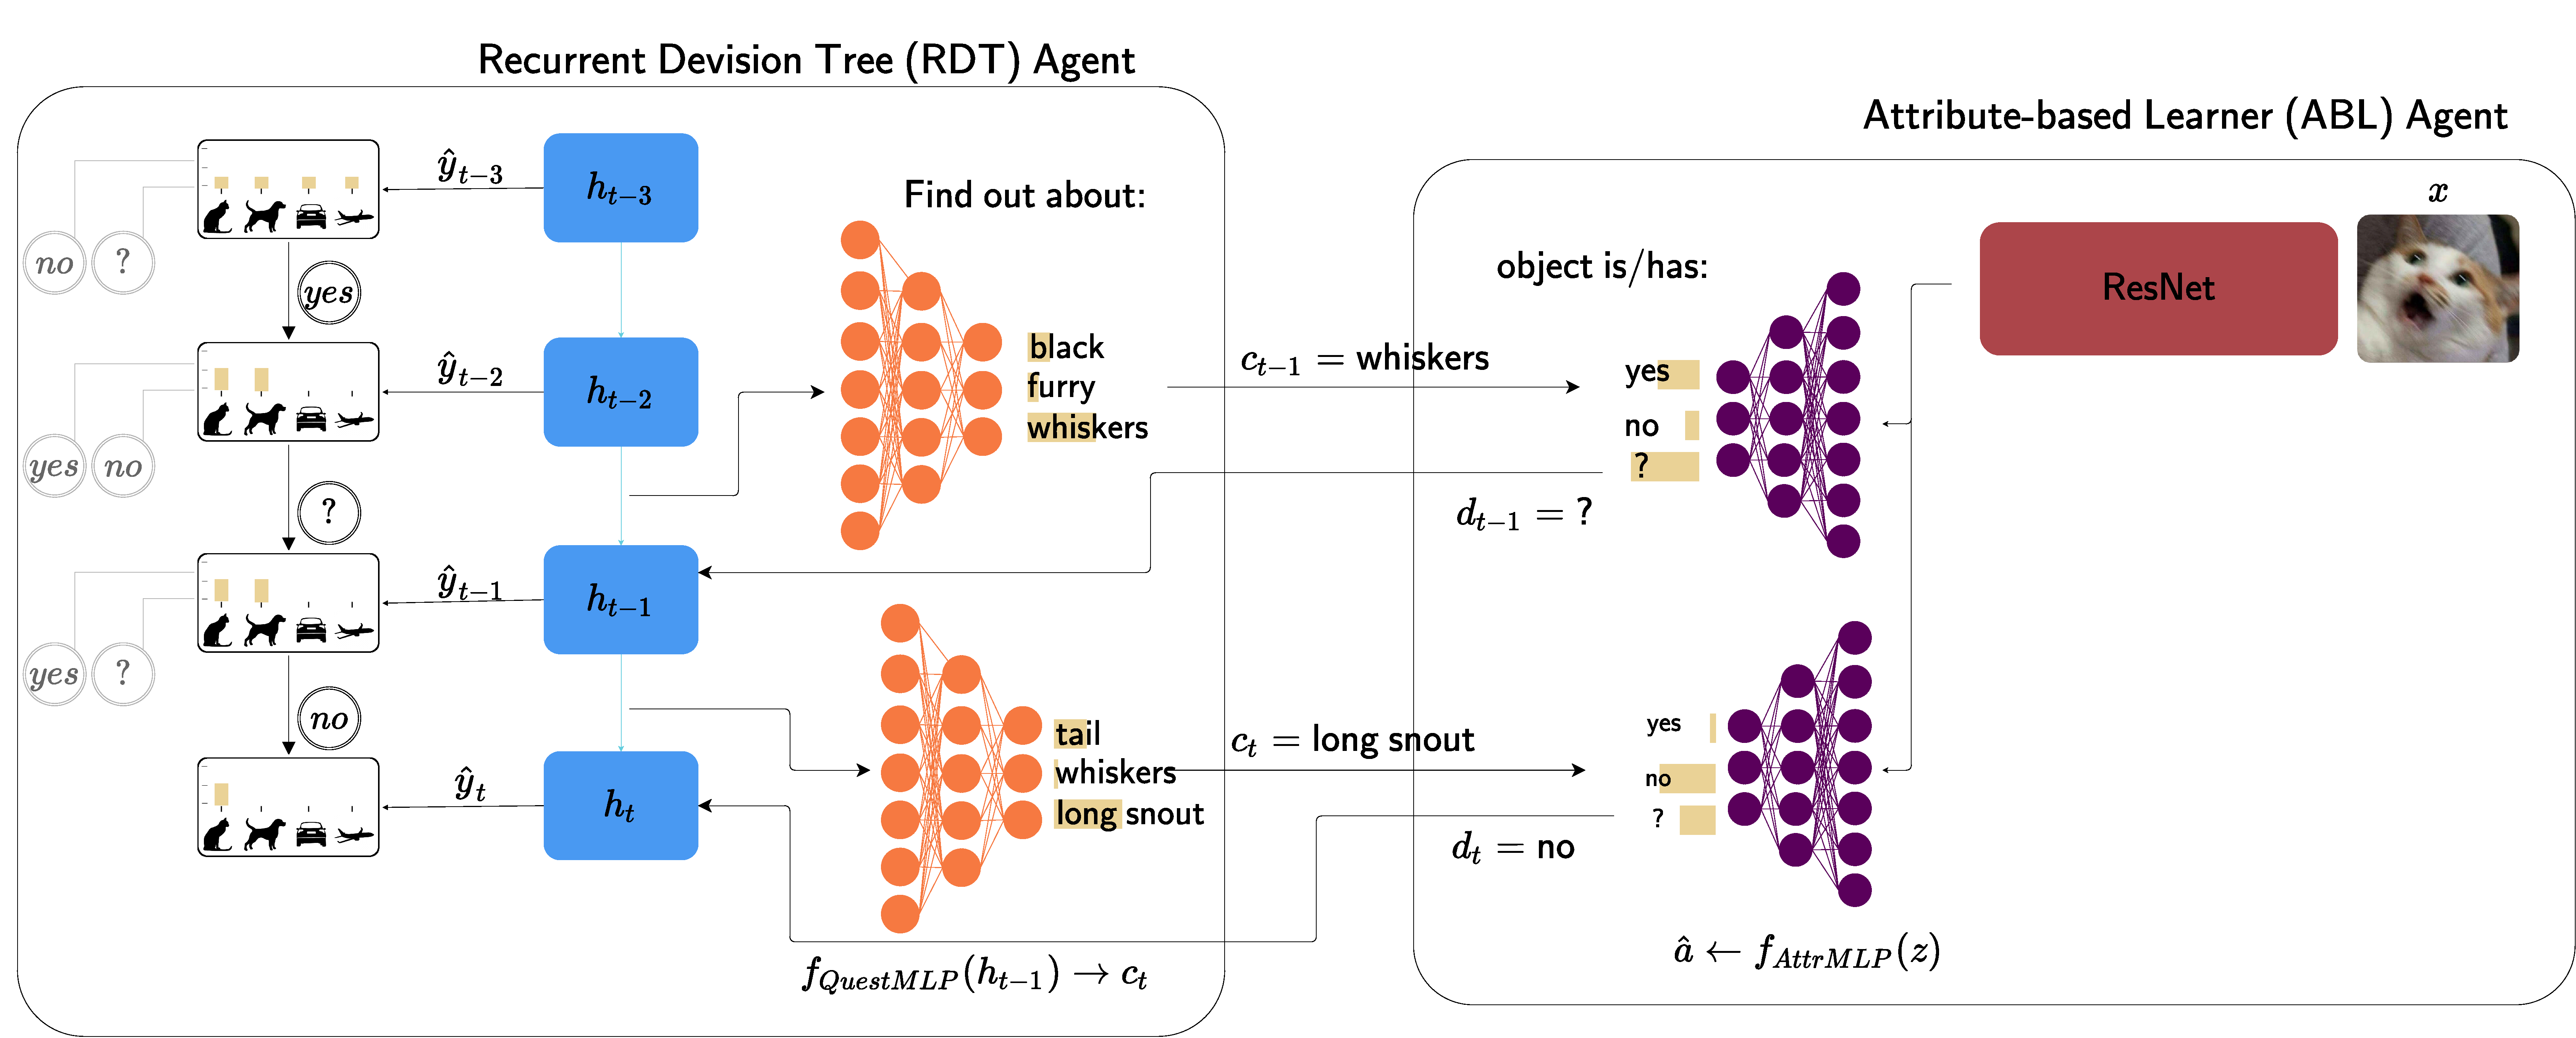
\includegraphics[width=1\textwidth]{images/uncertaintRDTC.pdf} 
	\caption{The RDT agent asks questions about presence, absence or uncertainty of attributes. The answers, given by the AbL agent are used by the RDT agent to make a classification each iteration.}
	\label{fig:uncertainRDTC}
\end{figure}

\section{RDTC} 
Before we introduce our modifications to the RDTC model, we will give a detailed explanation of its architecture, learning algorithm and how the two agents communicate.

%TODO intro
\subsection{Communication}
The two agents communicate to each other through discrete values. For a given image, the AbL returns a an answer $\hat{a}$ that is a tensor with binary values with size $\text{number of attributes} \times \text{decision size}$. The intention behind using only binary values in the AbL's answer is increased interpretability. Each row in this tensor indicates the presence/absence of an attribute and the columns correspond to the decision options 'Yes' or 'No'. Strictly speaking, the AbL thus answers all possible questions the RDT can ask,in advance to any questions. 
The RDT is then able to ask questions through posing an index $c_t$. By accessing the AbL's answer at this index it receives answer $d_t = \hat{a}[d_t]$. This information then used to build an internal decision tree, used for a classification output and to come up with a new question. In the following, we will go over each agent in more detail and explain how this model is trained.


\subsection{AbL}
The AbL agent is a vision model, consisting of a CNN and a MLP. The CNN learns image features and the MLP learns a mapping from features to human-annotated attributes (if available). For all experiments, we use a ResNet \cite{he2016deep} to extract features. For a given image $x$, the CNN extracts feature vector $z$. This is passed to the $f_{AttributeMLP}$ and the resulting vector of logits is put through a softmax. The output is a tensor $p(\hat{a}|z)$ with shape $number\_attributes \times decision\_size$. This corresponds to a probability distribution over the decision option for each attribute. In order to get an interpretable, binary response, in the forward pass, the result of the softmax is put through an arg max function. This is, however, not differentiable. In the backward pass it is therefore replaced by the identity function. Thus, the final response of the AbL agent for a given image $x$ is $\hat{a} = argmax(p(\hat{a}|z))$. The RDT agent can then access answers for specific attributes by indexing.


\subsection{RDT}
The RDT agent consists of several models. At its core lies an Long-short Term Memory (LSTM). This recurrent model allows the RDT to come up with new questions, based on it's hidden state $h_{t-1}$ from the last (or initial) communication step.\\
The $f_{QuestMLP}$ is responsible for thinking of new questions by returning an index that can be used to access attribute information in the response from $f_{AttributeMLP}$. The output of $f_{QuestMLP}$ is a categorical distribution $log\;p(c_t|h_{t-1})$ over possible indices $c_t \ in \lbrace 1,2,...,|A| \rbrace$. In order to get an actual index, the final output needs to be discrete. Thus we need to sample from this categorical distribution. This is done via the Gumbel softmax function:
\begin{align}
		GumbelSoftmax(log\;\pi) &= \frac{exp((log\;\pi_i + g_i)/\tau)}{\sum_{j=1}^{K}exp((log\;\pi_j + g_j)/\tau)}\text{ , where}\\
			log\;pi &=log\;p(c_t|h_{t-1})\text{ , and thus:}\\
			c_t &= GumbelSoftmax(log\;p(c_t|h_{t-1})).
\end{align}
where for $\tau \rightarrow 0$, the distribution approaches a one-hot vector with a $1$ at the maximum of the categorical distribution and $0$ everywhere else.\\ 
The resulting scalar $c_t$ then can be used to index $\hat{a}$. The response is $d_t$ which indicates absence, presence or uncertainty of the attribute at index $c_t$. Question $c_t$ and answer $d_t$ then update explicit memory $\mathcal{M}^{(t)} = \mathcal{M}^{(t-1)} \oplus (c_t, d_t)$. Note that during test time, rather than sampling $c_t$, the index with the highest probability is chosen.\\
The explicit memory $\mathcal{M}^{(t)}$, $c_t$, $d_t$ and the LSTM's last hidden state $h_{t-1}$ are then used to computer the current hidden state $h_t$, which is then, in turn, used by the $f_{QuestMLP}$ again to pose a new question.\\
The explicit memory $\mathcal{M}^{(t)}$ is also the basis for the class prediction. An additional MLP, the $f_{ClassMLP}$ returns class probabilities $\hat{y}_t$ based on  $\mathcal{M}^{(t)}$ for every communication step:
\begin{align}
	\hat{y}_t = f_{ClassMLP( \mathcal{M}^{(t)})}.
\end{align} The classification is the the final output of the model and is used to calculate a loss that can be optimized.


\subsection{Learning}
Ideally, the model should come to a classification in as few communication steps as possible. A tree resulting from few communication steps is shallow and easier to interpret. To keep the model from using deep trees, the classification loss is divided by the number of time steps (communication steps):
\begin{align}
	\mathcal{L} = \frac{1}{T} \sum_{t=1}^{T}\mathcal{L}_{CE}(y, \hat{y}_t) = - \frac{1}{T}\sum_{t=1}^{T}\sum_{i}y_i \cdot log\;\hat{y}_{t,i}.
\end{align}
This ensures, that the lower the number of time steps $T$, the lower the whole term and thus the lower the loss.\\
Besides the classification loss, an additional attribute loss can be leveraged in order to encourage learning attributes that correspond to provided human annotated side information.
\begin{align}
	\mathcal{L} = \frac{1}{T}\sum_{t=1}^{T}\left[(1-\lambda)\mathcal{L}_{CE}(y,\hat{y}_t) + \lambda \mathcal{L}_{CE}(\alpha_{y,c_t},\hat{\alpha}_{c_t}) \right]
\end{align}
How much each loss contributes to the total loss can be determined by hyperparameter $\lambda$.



\section{Uncertainty}


Uncertainty information is a crucial part of robust vision systems. In safety critical application, it could be avoided that the model uses high-risk strategies by leveraging attributes it is highly uncertain about for its classification. Or, if all attributes are deemed highly uncertain (for example on completely ood data), the model could decide to consult a human instead of making an overconfident classification.\\
Uncertainty comes either from variance in data (aleatoric uncertainty) or from variance in model parameters (epistemic uncertainty). Thus, there is an inherent relationship between variance and uncertainty.
%To get an intuition of the relationship between uncertainty and variance, let us have look at the basic equation for variance.
The variance of a random variable, which is in our case the variational predictive distribution $p(\hat{y} | x)$ with $y\sim p(\hat{y} | x)$, is defined as:
\begin{align}
	Var_q(p(\hat{y} | x)) &= \mathbb{E}_q \left[ (y-\mathbb{E}\left[ y\right])^2 \right]\\
	&= \mathbb{E}_q \left[yy^T\right]  - \mathbb{E}_q\left[y\right]\mathbb{E}_q\left[y\right]^T.
\end{align}
To decompose the term into variance arising from data and variance from the model $q$ itself, according to \citet{kwon2020uncertainty}, we can write it as:
\begin{align}
Var_q(p(\hat{y} | x)) &= \mathbb{E}_q \left[yy^T\right]  - \mathbb{E}_q\left[y\right]\mathbb{E}_q\left[y\right]^T\\
	&\underbrace{=\int_{\Omega}\left[ diag (\mathbb{E}_{p(\hat{y}|x,w)}[\hat{y}]) -\mathbb{E}_{p(\hat{y}|x,w)}[\hat{y}] \cdot \mathbb{E}_{p(\hat{y}|x,w)}[\hat{y}] \right]q_{\theta}(w)dw}_{aleatoric}\\
	&+\underbrace{\int_{\Omega}\left[ \mathbb{E}_{p(\hat{y}|x,w)}[\hat{y}] - \mathbb{E}_{q_{\theta}(\hat{y}|x,w)}[\hat{y}] \right] \left[ \mathbb{E}_{p(\hat{y}|x,w)}[\hat{y}] - \mathbb{E}_{q_{\theta}(\hat{y}|x,w)}[\hat{y}] \right]^T}_{epistemic}.
\end{align}









\subsection{Estimating Epistemic Uncertainty with Dropout Neural Networks}
Epistemic uncertainty corresponds to the variance of the models parameters.
In a traditional dropout neural network, there is no random dropping out of neurons in test stage and weights are fix. This would result in no variance of model outputs for multiple forward passes given an input. However, dropping out neurons in a random manner results in an inherent variance of model parameters. \citet{gal2016dropout} proof that this variance corresponds to epistemic (model) uncertainty. Here, we will go through their proof.\\
The key idea is that a dropout neural net is equivalent to an approximation of a Gaussian process. To randomly dropout neurons, we sample binary values that are either $0$ or $1$ for every neuron. The sampled value is then multiplied with the neurons value.
In the following, the dropout neural network with $L$ layers the weight matrices are denoted by $W_{l \in L}$, the bias vectors by $b_l$, the network output given datapoint $x_i \in X$ with size $N$ by $\hat{y}_i$, and the true value by $y_i \in Y$. The objective of the network is to minimize a given loss function $E(y_i, \hat{y}_i)$. Additionally, a weighted regularization term can be added to the loss function. A popular technique is to use $L_2$ regularization, weighted by a weight decay term $\lambda$. The final resulting loss term is:
\begin{align*}
\mathcal{L}_{dropout} := \frac{1}{N}\sum_{i=1}^{N}E(y_i, \hat{y}_i) + \lambda \sum_{l=1}^{L}(||W_l||^2_2 + ||b_l||^2_2).
\end{align*}
For the special case of a single hidden layer dropout network, we can rephrase this objective as
\begin{align}\label{eq:dropout}
\mathcal{L}_{dropout} := \frac{1}{N}\sum_{i=1}^{N}E(y_i, \hat{y}_i) + \lambda (||W_1||^2_2 + ||W_2||^2_2+ ||b||^2_2)
\end{align}, where $W_1$ is the weight matrix connecting the input to the hidden layer, and $W_2$ connecting the hidden to the output layer. The bias $b_2$ 
Let us take a step back to a very general point of view. A problem, we typically encounter in machine learning is how to predict a function value $y^*$ from a datapoint $x^*$. In Bayesian terms, we want to find the predictive posterior
\begin{align}\label{eq:pred_post}
 p(y^*|x^*, X,Y) = \int p(y^*|x^*, w)p(w|X,Y)dw
\end{align}

where $w$ is a set of adjustable parameters. In order to model our function of interest well, we need to find optimal values for $w$. If we break down Equation \ref{eq:pred_post} further, we get
\begin{align}
p(y^*|x^*, X,Y) = \int \underbrace{p(y^*|x^*,w)}_{\mathcal{N}(\underbrace{y;\hat{y}(x,w)}_{\hat{y}(x, w=\lbrace W_1, W_2,...,W_n\rbrace)},\tau^{-1}\mathbf{I}_D)} \cdot \hspace{15pt}\underbrace{p(w|X,Y)}_{intractable}dw
\end{align}
, where we see that the posterior over $w$, given data is intractable. Therefore we need to approximate it with variational distribution $q_{\theta}(w)$. We want this distribution to mimic the true posterior closely. Therefore, we want to find
\begin{align*}
	argmin_{\theta} KL(q_{\theta}(w)|p(w|X,Y))
\end{align*}
As we have seen in Section \ref{sec:vi}, this would require access to the true posterior, which we cannot compute. Therefore we maximize the log evidence lower bound
\begin{align*}
\mathcal{L}_{VI} := \int q_{\theta}(w) log p (Y|X, w)dw - KL(q_{\theta}(w)||p(w))
\end{align*}
and assume $p(w)$ to be a standard Gaussian. As discussed also in Section \ref{sec:vi}, we effectively turn computing integrals into an optimization problem, where we need to compute derivatives. Using the optimized variational distribution $q_{\theta}^*(w)$, we can compute an approximate predictive posterior 
\begin{align*}
q_{\theta}(y^*|x^*) = \int p(y^*|x^*, w)q_{\theta}^*(w)dw
\end{align*}
for a given datapoint $x^*$. This in turn can be approximated with
\begin{align*}
q_{\theta}(y^*|x^*) = \sum_{t=1}^{T}p(y^*|x^*, w_t)
\end{align*}
where each $w_t$ is a sample from our variational distribution $p_{\theta}^*(w)$.
\\
Now, in Gaussian processes, as discussed in Section \ref{sec:gp}, we need a covariance function of the form 
\begin{align*}
K(x,y) = \int \mathcal{N}(w;0, l^{-2} I_Q)p(b)\sigma(w^Tx+b)]sigma(w^Ty +b)dwdb
\end{align*}
to get a covariance matrix. To avoid computing integrals, this covariance function can be approximated with
\begin{align*}
	\hat{K}(x,y) = \frac{1}{K} \sum_{K}^{k=1} \sigma(w^T_k x + b_k)\sigma(w^T_k y + b_k)
\end{align*}
where $w_k$ is sampled from $\mathcal{N}(0, l^{-2}I_Q)$ and $b_k$ from $p(b)$. This is called Monte-Carlo integration \cite{metropolis1949monte}.\\
This gives us following predictive posterior for our GP:
\begin{align*}
w_k \sim \mathcal{N}(0, l^{-2}I_Q), w_d \sim \mathcal{N}(0, l^{-2} I_K), b_k \sim p(b)\\
W_1 = \left[ w_k \right]^{K}_{k=1}, W_2 = \left[ w_d \right]^D_{d=1}, b = \left[ b_k \right]^K_{k=1}, w = \lbrace W_1, W_2, b \rbrace\\
p(y^*|x^*, w) = \mathcal{N} \left( y^*; \sqrt{\frac{1}{K}\sigma(x^* W_1 + b)W_2, \tau^{-1}I_N}\right)\\
\text{,and finally:}\hspace{150pt}\\
p(y^*|x^*, X,Y) = \int p(y^*|x^*, w)p(w|X,Y)dw.
\end{align*}
%TODO note that this is for normal GP and single hidden layer dropout net
We use $q_{\theta}(w) = q_{\theta}(W_1)q_{\theta}(W_2)q_{\theta}(b)$ as an approximation to $p(w|X,Y)$, where
\begin{align}\label{eq:gaussian_mixture}
q_{\theta}(W_1) = \Pi q_{\theta}(w_q), \text{ and } q_{\theta}(w_q) = p_1\mathcal{N}(m_q, s^2, I_K) + (1-p_1) \mathcal{N}(0, s^2, I_K),\\
\text{ with } p_1 \text{ as a probability }\in \left[ 0, 1\right], s > 0, \text{ and }M_1 = \left[ m_q \right]^Q_{q=1} \in \mathbb{R}^{K\times D}
\end{align}
We eventually want to recover a dropout neural network (as specified in Eq. \ref{eq:dropout}) from our GP. In our dropout network we rely on sampling from a Bernoulli random variable. In our GP, we, so far, sample from a mixture of Gaussian distributions. We cannot change this, because the KL-divergence between a discrete distribution (Bernoulli) and a continuous distribution (Gaussian) is not defined. Therefore we will make two assumptions about the Gaussian mixture in Eq. \ref{eq:gaussian_mixture}.\\
We set $p$ to a fix value. Also, we want the second term of the sum to be zero. To sample zero from a zero-centered Gaussian distribution with a very high probability, we simply set the standard deviation to a very small value. Small enough, so that a device with limited precision will view it as zero and always return zero. These two assumptions leave us with a Gaussian distribution that resembles a Bernoulli distribution. Thus, we are effectively sampling from a Bernoulli random variable in our GP, with a still defined KL-divergence. We get
\begin{align*}
\mathcal{N}_{GP-MC} \approx log p(Y|X, \hat{w}) - \frac{p_1 l^2}{2} ||M_1||^2_2 - \frac{p_2 l^2}{2}||M_2||^2_2 - \frac{l^2}{2}||m||^2_2 \text{, with } \hat{w} \sim q_{\theta}(w)
\end{align*}
as approximated log evidence lower bound.
% here, the maximizing variational parameters are the same as in the ELBO specified, above
To recover the dropout objective from Eq. \ref{eq:dropout}, we can scale it by a constant $\frac{1}{N \tau}$.
\begin{align*}
\mathcal{L}_{GP_MC} \propto  - \frac{1}{2N} \sum_{n=1}^N ||y_n - \hat{y}_n||^2_2 -  \frac{p_1 l^2}{2N\tau} ||M_1||^2_2 - \frac{p_2 l^2}{2N\tau}||M_2||^2_2 - \frac{l^2}{2N\tau}||m||^2_2
\end{align*}
and set hyperparameters $\tau$ and $l$ to appropriate values.


\subsection{Getting Uncertainty Information}
\begin{figure}
	\centering
	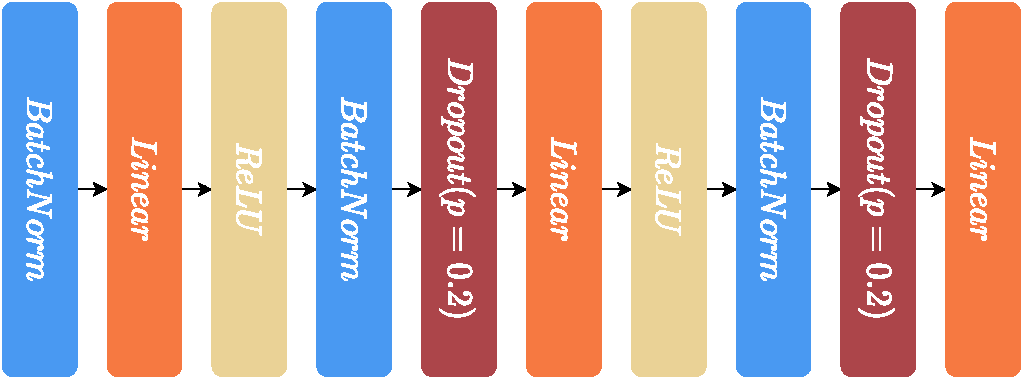
\includegraphics[width=0.9\textwidth]{images/f_attrMLP.pdf} 
	\caption{We used both BatchNorm and dropout layers for $f_{attrMLP}$.}
	\label{fig:f_attrMLP}
\end{figure}
We tested different configurations for $f_{AttributeMLP}$ and using a combination of dropout and batchnorm layers between, fully connected layers and non-linearities worked best. This setup is displayed in Figure \ref{fig:f_attrMLP}. To retrieve uncertainty information, given the image features $z$ from the ResNet, we do $n$ forward passes and compute the standard deviation of the results. As proofed by \citet{gal2016dropout}, this is equal to epistemic uncertainty. So theoretically, for examples, that are far from the distribution, the model was trained on, it should yield high epistemic uncertainty. 
After retrieving uncertainty information, we replace selection logits from $f_{QuestMLP}$ that are on indices with high uncertainty by $-inf$ so they can not be picked by the Gumbel softmax. We call this strategy remove uncertain attributes (remRDTC). In another strategy, uncertain attributes are denoted with a $1$ in a extended decision tensor. We refer to  as extended vocabulary (extRDTC).


\subsection{Removing Uncertain Attributes}\label{sec:remRDTC}
%\begin{figure}[t!]
%	\centering
%	\begin{minipage}{0.45\textwidth}
%		\centering
%		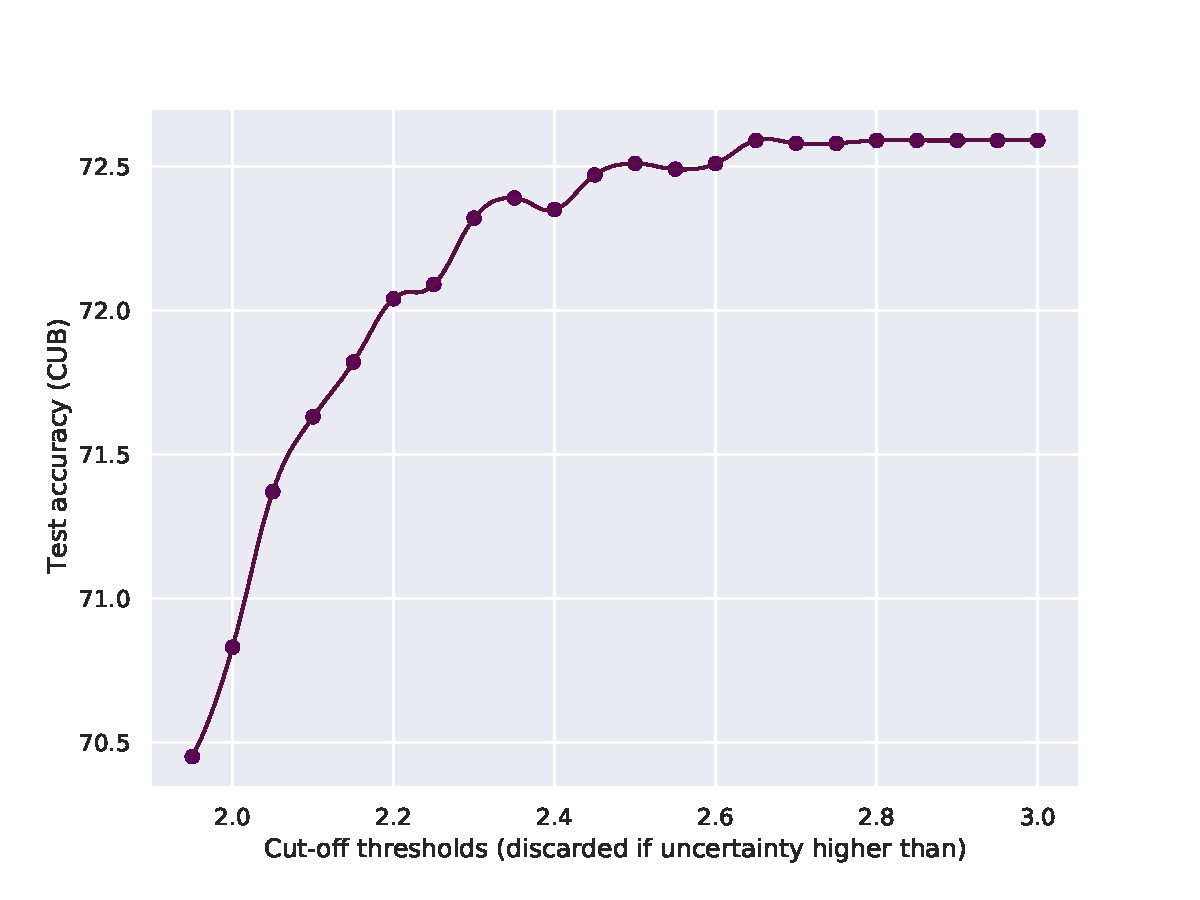
\includegraphics[width=1\textwidth]{images/threshold_accuracy.pdf} 
%		\caption{Test accuracies, when removing uncertain attributes with different thresholds. Note, that here we used a model that was trained for 30 epochs and used max\_iters=20.\\\hspace{40pt}}
%		\label{fig:threshold_accuracies}
%	\end{minipage}\hfill
%	\begin{minipage}{0.45\textwidth}
%		\centering
%		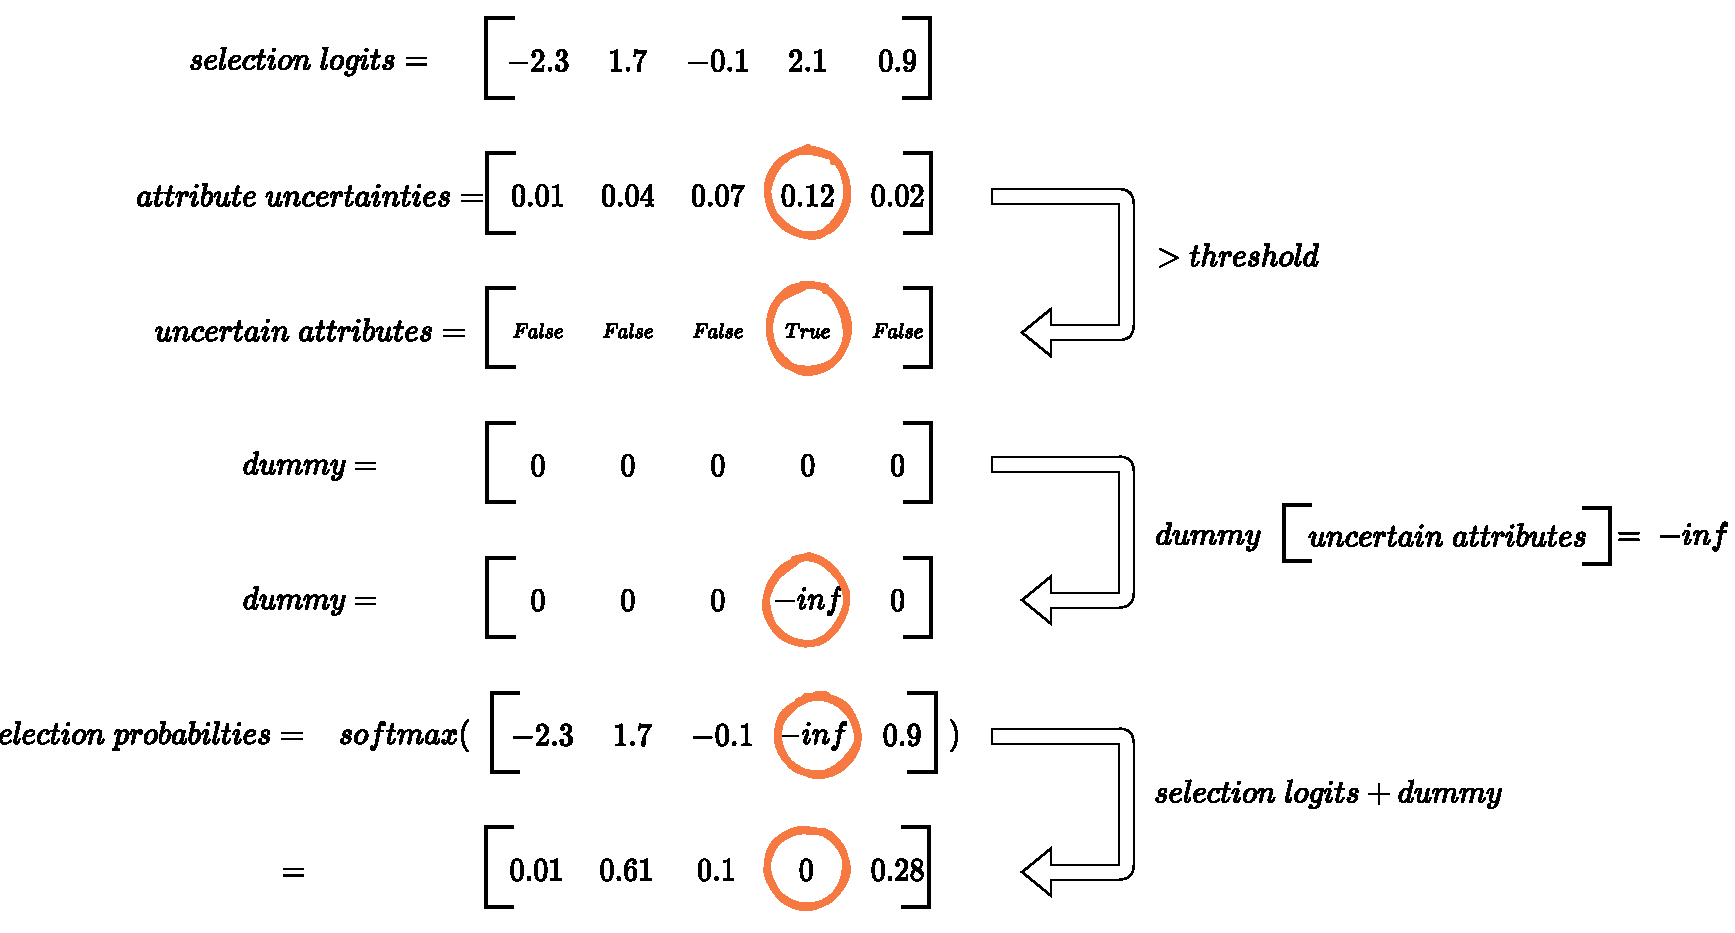
\includegraphics[width=1\textwidth]{images/remove_attrs.pdf}
%		\caption{...}
%		\label{fig:remove_intuition}
%	\end{minipage}
%\end{figure}
\begin{figure}
	\centering
	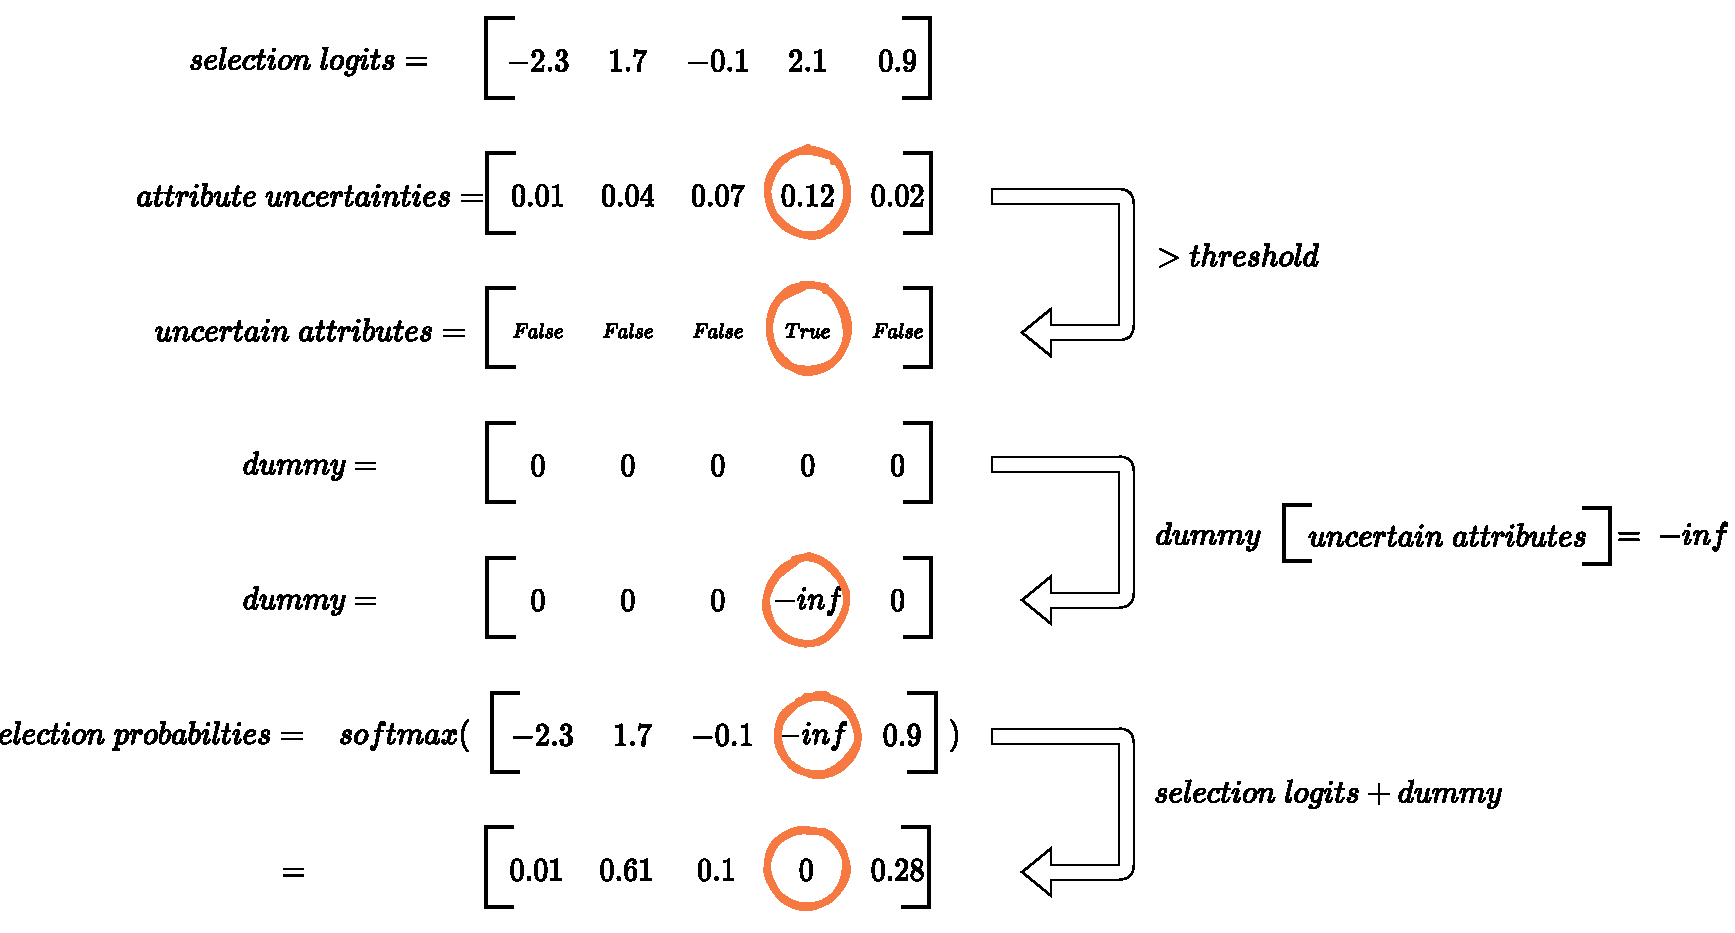
\includegraphics[width=0.8\textwidth]{images/remove_attrs.pdf} 
	\caption{In selection logits, the output from $f_{QuestMLP}$, we replace values at indices where uncertain attributes are with a $-inf$ value. This assures that this attribute can never be picked as $c_t$ by the Gumbel softmax.}
	\label{fig:remove_intuition}
\end{figure}

%TODO rewrite
After calculating uncertainty for each attribute, in this strategy, we simply manipulate the logits tensor from $f_{QuestMLP}$ so that at each index, where a uncertain attribute is, the selection logit tensor has a -inf value. This ensures that this attribute cannot be picked by the Gumbel softmax. In turn, no uncertain attribute can be picked as index and therefore cannot be posed as a question to the AbL.\\
In order to prevent the model from misusing uncertainty information, we have to ensure that the model does not get any gradients where uncertain attributes are.

%We tested this strategy both in test-only and in training and testing stage. When using it in the test stage for a model, that was trained regularly (without uncertainty information), the model suffered severe performance drops, displayed in Figure \ref{fig:threshold_accuracies}. Especially, for low cut-off thresholds. It never outperforms a model that keeps all attributes. We hypothesize that this is due to actively removing options from a pool of attributes, that the model is already well adapted to and as shown in Figure \ref{fig:less_attrs} rarely misclassifies despite being uncertain.



\subsection{Extending the Vocabulary}
Here, we resort to an extended vocabulary of answers for $f_{AttrMLP}$. Instead of just allowing $Yes$ and $No$, we also allow the AbL to answer with $?$. Thus, $f_{AttrMLP}(z) \in \lbrace 0,1 \rbrace^{num\_attributes \times 3}$. However, since, $f_{AttrMLP}(z) \in \lbrace 0,1 \rbrace^{num\_attributes \times 2}$ we need to append the uncertainty information to $d$ while avoiding conflicting answers. This process is shown, for a two attribute example in Figure \ref{fig:extended_vocab}. After receiving the output from $f_{AttrMLP} = d_{init}$ we initiate the uncertain column $?$ with a vector of $0$s and append this to the $d_{inint}$ to create $d_{temp}$. After computing uncertainty vector $?$, we also create a negated version $!$ of it. This indicates all attributes where the model is certain. Subsequently, those are now used to clear rows. Vector $!$ has $0$s where the model is uncertain. We use this to replace values in rows of uncertain attributes with $0$s and get $d_{cleared}$. We also initiate a dummy tensor, that is of the same dimension as the $d_cleared$ and is all $0$s but in the column to the very right, where it is all $1$s. Rows of this tensor are now cleared, using $?$, wherever $?$ has zeros, thus only rows with uncertain attributes remain and have a $1$ in the column responsible for uncertainty. Finally, this tensor, and $d_cleared$ are added up to create our final decision $d$ which can now be indexed by the RDT.\\
When using this strategy in training, we need to make sure, that no gradients actually come from uncertainty, so it is not misused and maximized in order for the model to profit from the additional column. We need to ensure that gradients only come from attributes, where the model is certain. For the operation, as described above, this is the case. We detach $?$ and $!$ from the computational graph. The dummy tensor is a leaf node, so no gradient is computed. Also, where values  in $d$ are $0$, their activation's derivative is $0$, so gradients are $0$. This is the case in rows of uncertain attributes. Which gradients are used and which are blocked in the previously used example is displayed in Figure \ref{fig:extended_vocab_backward}.

\begin{figure}[t!]
	\centering
	\begin{minipage}{0.45\textwidth}
		\centering
		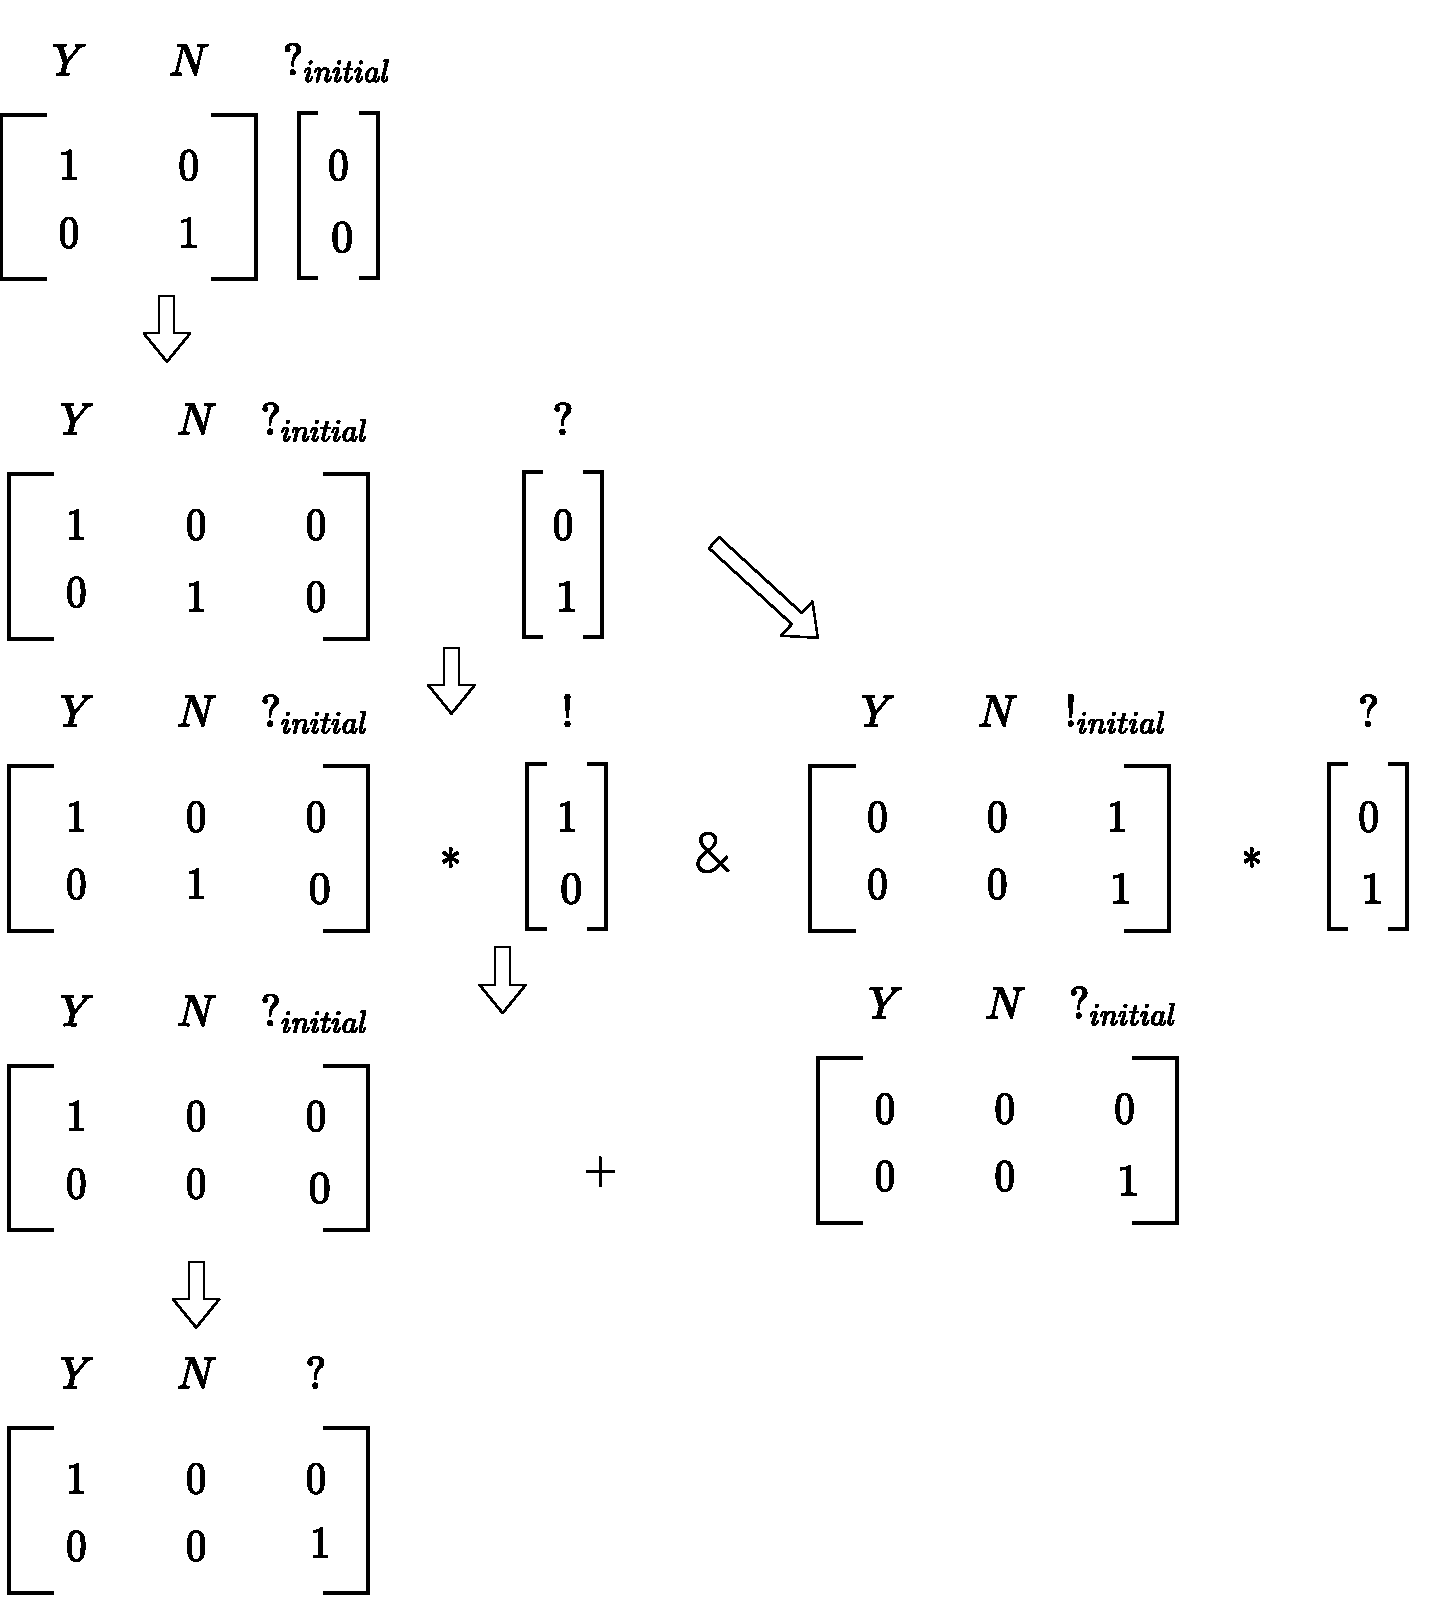
\includegraphics[width=1\textwidth]{images/extended_vocab.pdf} 
		\caption{The original answer by the AbL is merged with uncertainty information so that the answer for each attribute is either 'yes', 'no' or '?'. Here we show a small example where attribute size is only $2$.}
		\label{fig:extended_vocab}
	\end{minipage}\hfill
	\begin{minipage}{0.45\textwidth}
		\centering
		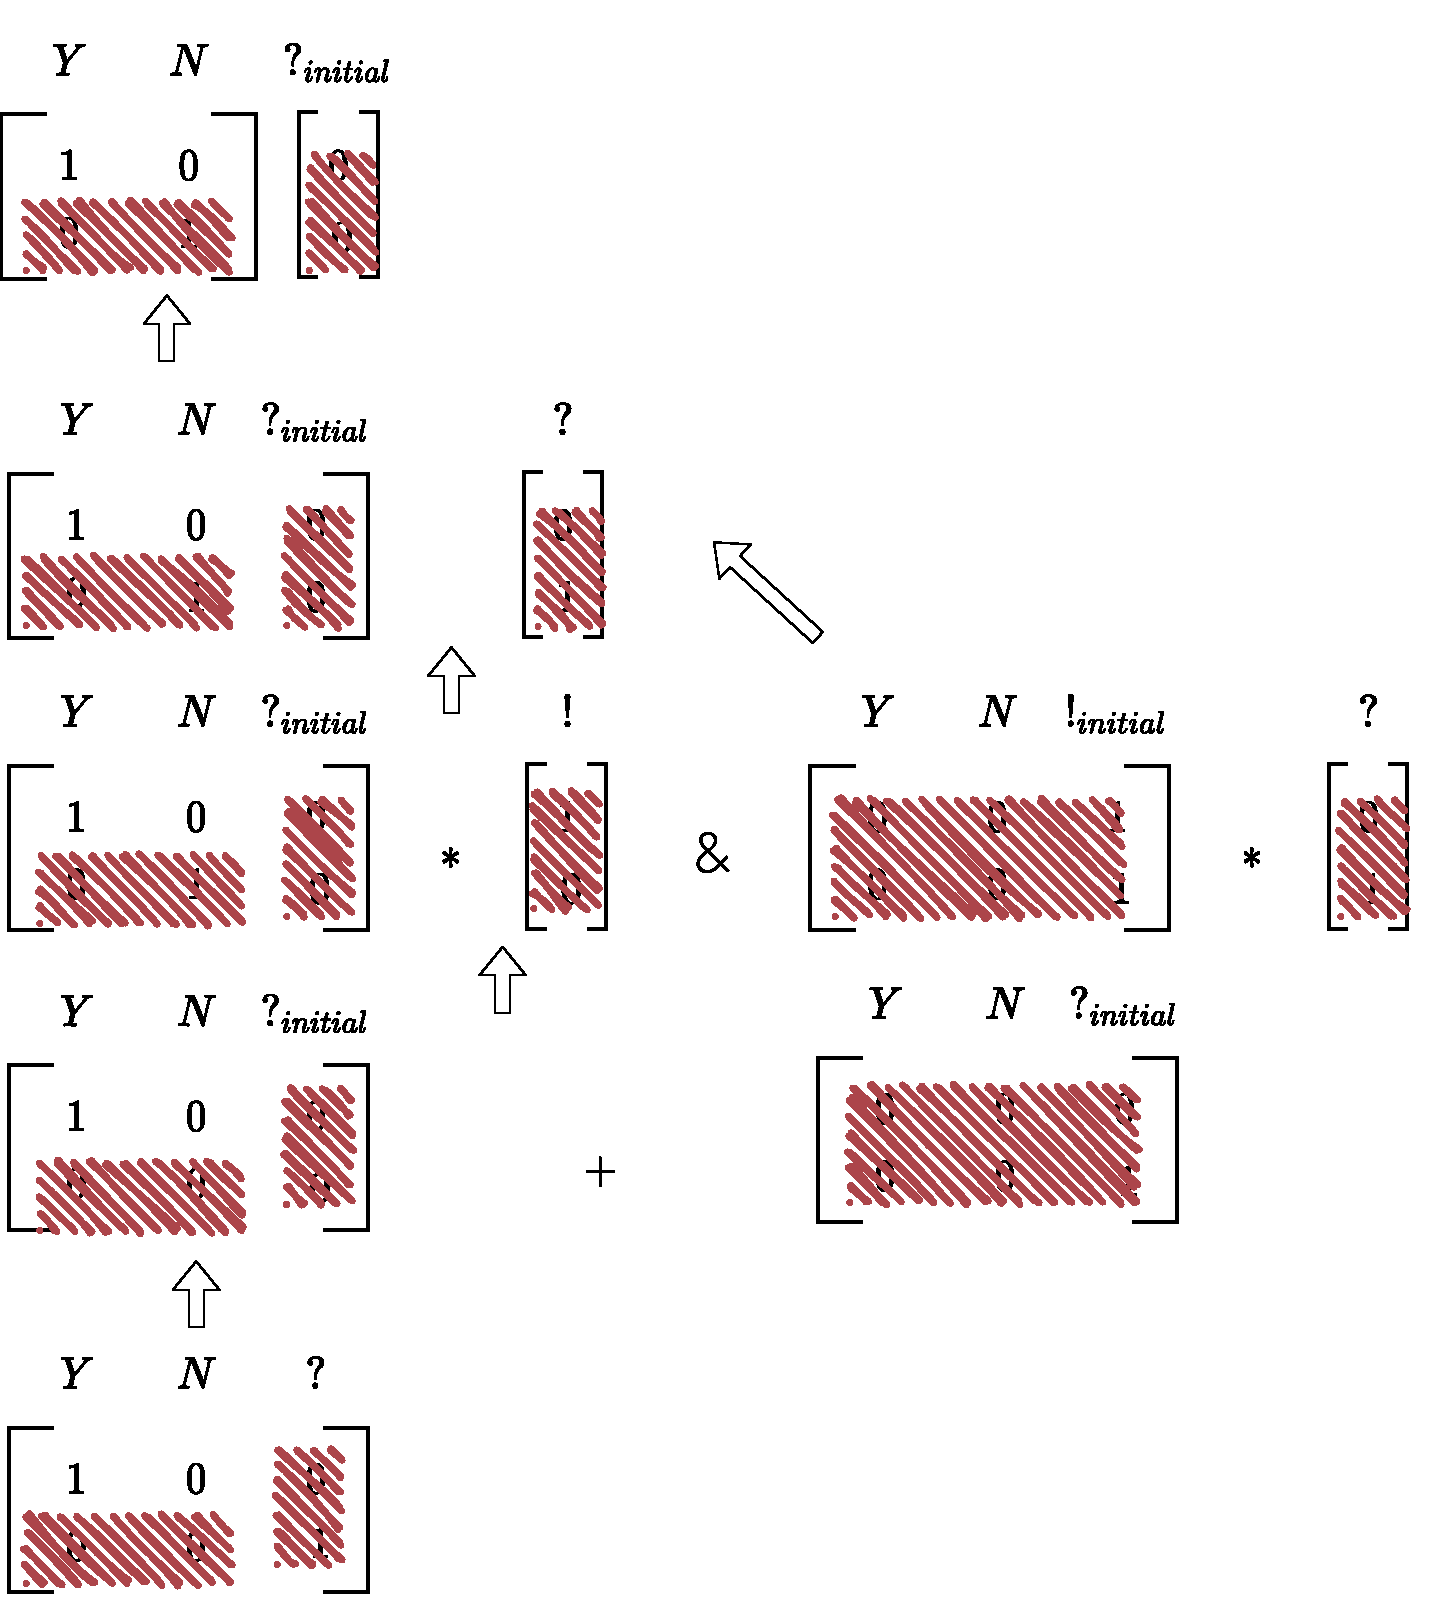
\includegraphics[width=1\textwidth]{images/extended_vocab_backward.pdf}
		\caption{Gradients coming from attributes that are deemed uncertain are detached from the computational graph. Other elements in the tensor are either $0$ (so are their respective gradients), or stem from leaf nodes.}
		\label{fig:extended_vocab_backward}
	\end{minipage}
\end{figure}


\subsection{Random Attribute Removal}
Similar to the remRDTC strategy, described in Subsection \ref{sec:remRDTC}, we prevent the RDT from asking questions. However, instead of blocking indices where uncertain attributes are, we randomly generate a tensor and block indices based on it. The probability of an index being blocked is similar to the probability of an attribute being deemed uncertain to allow fair comparison.


\chapter{Experiments}
We evaluated our proposed model on different image classification datasets which provide attributes as side information. We also investigate the models behavior by quantitatively analyzing uncertainties and their affects.


\section{Datesets}
We test our model on image datasets that provide attributes as side information. Popular datasets for this setting are Animals with Attributes 2 (AwA2) \cite{8413121}, aPY \cite{farhadi2009describing} and CUB \cite{WahCUB_200_2011}. Datasets with attributes are frequently used for zero- or few-shot learning tasks. In the explainable machine learning community they are popular since attributes provide a human interpretable, natural language parametrization of features.\\
%TODO describe datasets in more detail
AwA2 is a set of 37,322 images that can be subdivided into 50 different classes of animals. Human annotators were tasked to label each image, choosing from 85 available attributes that describe each animal class. The aPY dataset provides 15,339 images, annotated with 64 different attributes that describe each of the 32 classes. Finally, the most challenging dataset is CUB. Here, the task is to classify 11,788 different images into 200 different classes. For this task, each images is annotated with 312 descriptive attributes.

\begin{figure}[t!]
	\centering
	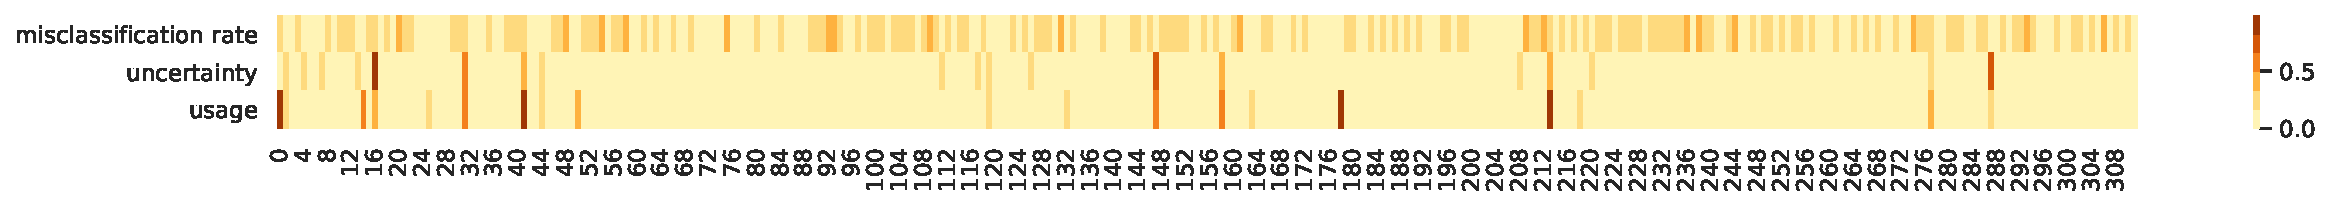
\includegraphics[width=1\textwidth]{images/attr_heatmap.png} 
	\caption{Normalized attributes misclassification frequency, uncertainty and usage. Only a small subsets of attributes is actually used by the model.}
	\label{fig:all_attrs}
\end{figure}
\begin{figure}[t!]
	\centering
	
\includegraphics[width=1\textwidth]{images/attr_heatmap_short.png} 
	\caption{Here, we only show normalized attributes misclassification frequency, uncertainty and usage for attributes that are used by the model.}
	\label{fig:less_attrs}
\end{figure}
\section{Statistics on Uncertainty}
The purpose of the proposed model is not only to evaluate it on benchmark datasets but also to quantitatively investigate uncertainties in the model and the data. We examined correlations between variables such as attribute uncertainty, usage and misclassificaion on the CUB dataset. From Figure \ref{fig:all_attrs} it becomes obvious that only a small subset off attributes as actually used to make decisions. We can already see, that most of the attributes that are used, however, are rarely misclassified. This is also visible in Figure \ref{fig:less_attrs} where only attributes that are used in the decision tree are shown. As apparent in the top row, all attributes here are classified correctly quite reliably. However, there seems to be no obvious correlation between uncertainty and misclassification as among the frequently used attributes (and thus reliably classified correctly) there are some attributes that have high uncertainty values.\\
In Figure \ref{fig:correlations} we can see that this is true and uncertain attributes appear among all levels of attribute accuracy. Figure \ref{fig:corr_matrix} proves further proofs this as the correlation between the two is close to $0$. It also shows high negative correlation between attribute misclassification frequency and usage. We can view misclassification frequency as inverse accuracy and thus have a positive correlation of $0.5$ between usage and accuracy, suggesting that the model actively avoids attributes that it is likely to classify.


\begin{figure}[t!]
	\centering
	\begin{minipage}{0.45\textwidth}
		\centering
		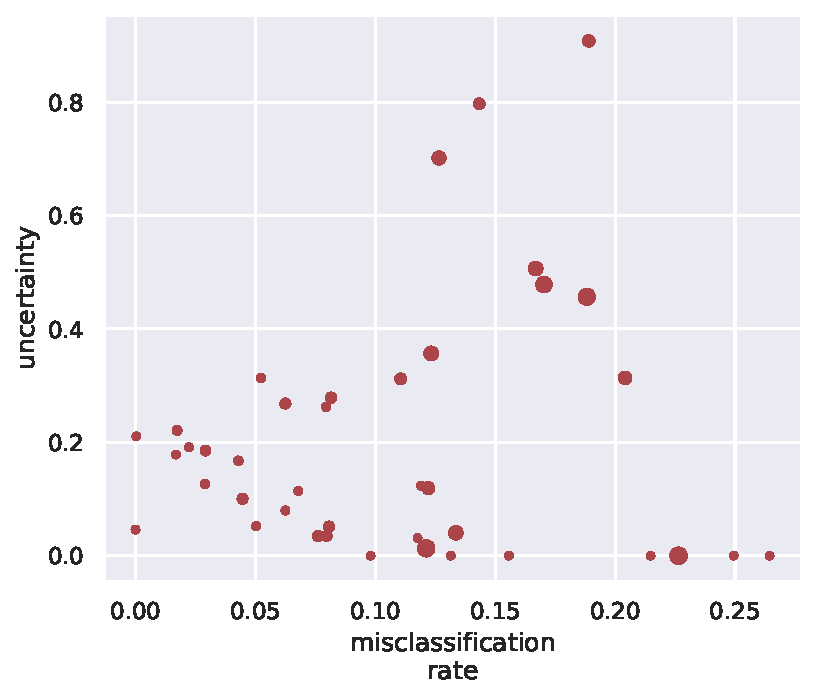
\includegraphics[width=1\textwidth,height=0.16\textheight]{images/error_sigma_corr_all.png} 
		\caption{...}
		\label{fig:correlations}
	\end{minipage}\hfill
	\begin{minipage}{0.45\textwidth}
		\centering
		
\includegraphics[width=0.8\textwidth,height=0.16\textheight]{images/corr_matrix.png}
		\caption{...}
		\label{fig:corr_matrix}
	\end{minipage}
\end{figure}

\section{Testing on Out-of-domain Data}\label{sec:zero_shot}
An important aspect of our model is that it is not only self aware regarding uncertainty, but also allows for human introspection. Here, we test whether examples, far from the training data, the model has seen cause high uncertainty. We use a attribute-zero-shot setting, where we exclude certain classes from training data, so that some attributes are never seen by the model in training. For our setting, we use the CUB dataset, as it is the most challenging out of the introduced three.\\
A classical zero-shot setting or a generalized zero shot setting (both described by \cite{8413121}) would not yield meaningful insights here. As in our proposed model, we only consider epistemic attribute uncertainty, uncertainty of classes should only depend on whether attributes attributes have been seen by the model and not whether classes have seen by the model, a possible weakness of our model, we further discuss in \ref{sec:attr_uncertainty}. We want to construct a setting, where certain attributes do not occur in training data, and thus have to find classes, that have exclusive attributes. In CUB, we find a set of 24 classes that posses 5 attributes that do not occur in any of the other classes\footnote{This setting can be replicated by using the \textit{zero\_attr\_train\_test\_split.txt} file in the provided Github repository.}.\\
After training our model on the proposed split, we investigate (1) uncertainties of classes that contain unseen attributes (Figure \ref{fig:unseen_attr_classes}) and (2) uncertainties of the unseen attributes themselves (Figure \ref{fig:unseen_attrs}). For (1), we computed the mean uncertainty per example. For (2), we consider all uncertainty values of each attribute.
We observe that the 24 classes, possessing unseen attributes have a overall higher uncertainty. Figure \ref{fig:unseen_attr_classes} displays the modeled distribution of mean uncertainty per example, divided into classes that only posses attributes, occurring in the training data, and classes that posses 5 attributes, never encountered during training. We observe, that the latter have a overall higher uncertainty.\\
Displayed in Figure \ref{fig:unseen_attrs}, is the distribution of uncertainty values of attributes available during training, and the uncertainty values of attributes, unseen by the model, before the test stage. Here, we also observe an overall higher uncertainty for the latter.




\begin{figure}[t!]
	\centering
	\begin{minipage}{0.45\textwidth}
		\centering
		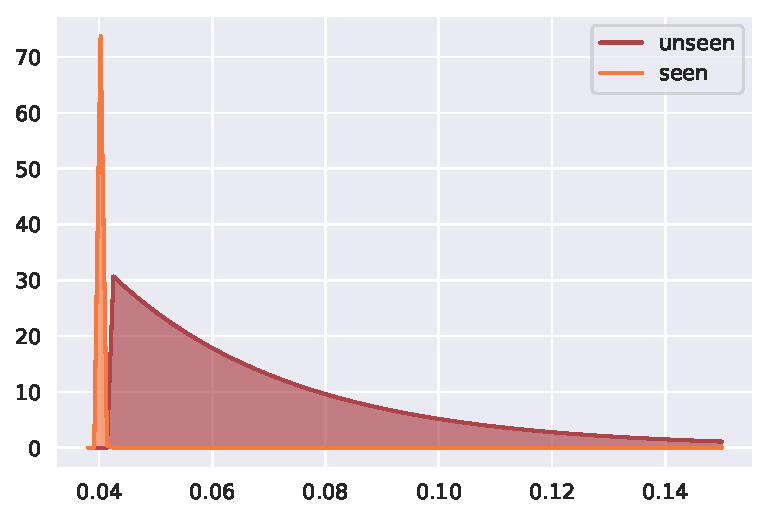
\includegraphics[width=1\textwidth]{images/zero_shot_class_uncertainty.pdf} 
		\caption{Exponential maximum likelihood model for uncertainty per example. Examples from classes that have unseen attributes have higher attribute uncertainties.}
		\label{fig:unseen_attr_classes}
	\end{minipage}\hfill
	\begin{minipage}{0.45\textwidth}
		\centering
		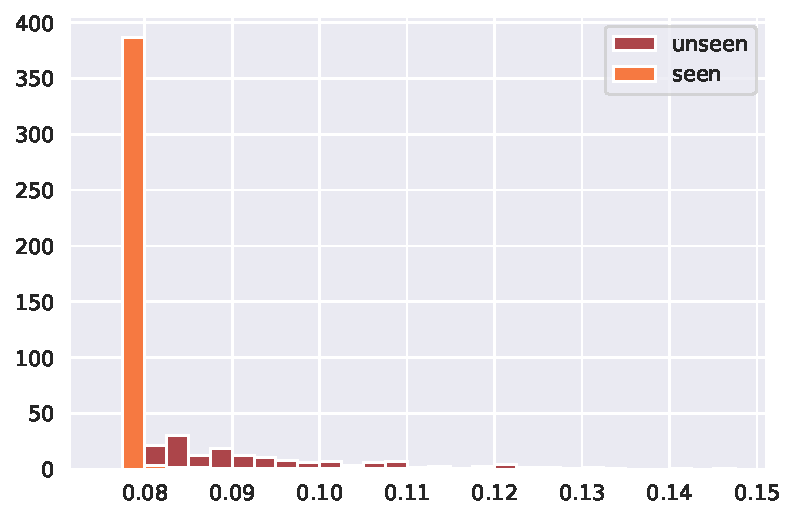
\includegraphics[width=1\textwidth]{images/zero_shot_attr_uncertainty_hist.pdf}
		\caption{Distribution of uncertainty values of seen and unseen attributes in zero-shot-attribute setting (See Section \ref{sec:zero_shot}). The model is more uncertain about attributes it has not encountered in the training set.}
		\label{fig:unseen_attrs}
	\end{minipage}
\end{figure}


\section{Results}\label{sec:results}
We compare our model to different other approaches, that either exemplify the current state of the art or are explainable.\\
ResNet-152 \cite{he2016deep} is not explainable. Here, the ResNet was pre-trained on ImageNet data \cite{deng2009imagenet} data and then fine-tuned on the specific tasks. We also use the ResNet trained in this manner in our proposed uRDTC model to extract features. When we train the uRDTC model, we keep the weights in the ResNet fixed and only adjust all other parameters in the model.
XDT and DT are both traditional decision tree models that serve as as a baseline. For DT \citet{alaniz2019explainable} propose following method: DT is are given features extracted by the previously introduced pre-trained ResNet. Splits are created according to values in extracted feature vector. For each split, one feature is chosen and then a split gets created. This is repeated until either each leaf node corresponds to exactly one class or a early stopping-criterion is met. Moreover, \citet{alaniz2019explainable} introduce XDT, where each split is given a semantic meaning, in order for the splits to correspond to interpretable attributes and not only features. The XDT is therefore not given features, directly stemming from the ResNet, but attributes, learned by a MLP that was trained to predict attributes given ResNet features. They train both DT and XDT using the CART algorithm \cite{breiman1984classification}. As splitting criterion, they chose the Gini impurity index over entropy-based methods due to its computational advantage \cite{raileanu2004theoretical}.\\
Another explainable model is Deep Neural Decision Forest (dNDF), proposed by \citet{kontschieder2015deep}. They learn an ensemble of trees by optimizing routing probabilities in each trees internal nodes. Every path through a tree eventually leads to class distribution, represented in leaf nodes. All internal nodes are sigmoid-activated, differentiable stochastic functions, parameterized by a optimizable $\theta$. The final prediction is an average over the resulting decision tree forest. On downside of the resulting averaged stochastic routing decisions is the reduced interpretability as they allow for multiple possible routes. The RDTC models only yield on possible route for a given example. Therefore, we consider only dNDF using a single tree instead of an ensemble mean.
\\



\subsection{Comparing RDTC to Other Models}
%$\rightarrow$\\
%\textit{Dataset}\\
%$\downarrow$\textit{Model}
\renewcommand{\arraystretch}{1.3}
\begin{tabular*}{\textwidth}{c @{\extracolsep{\fill}} c c c c}
	%\hline
	&                                AWA2&          aPY&          CUB\\
	\hline
	\hline
	ResNet \cite{he2016deep}&       $98.2\pm 0.0$& $85.1\pm 0.6$ & $79.0\pm 0.2$ \\ 
	\hline 
	DT&                             $78.0\pm 0.4$&$64.3\pm 0.6$  & $19.3\pm 0.3$  \\ 
	\hline 
	dNDF\cite{kontschieder2015deep}&$97.6\pm 0.2$&$85.0\pm 0.6$ & $73.8\pm 0.3$ \\ 
	\hline 
	RDTC\cite{alaniz2019explainable}&$98.0\pm 0.1$&$85.7\pm 0.7$& $78.1\pm 0.2$   \\ 
	\hline 
	XDT&                            $73.9\pm 0.9$&$59.9\pm 1.5$  & $4.9\pm 1.3$ \\ 
	\hline 
	aRDTC\cite{alaniz2019explainable}&$98.1\pm 0.0$&$85.3\pm 0.3$  &  $77.9\pm 0.6$\\ 
	\hline
	remRDTC(ours)&          $0.0\pm 0.0$          &          $0.0\pm 0.0$&  $0.0\pm 0.0$\\ 
	\hline
	extRDTC(ours)&          $0.0\pm 0.0$          &          $0.0\pm 0.0$&  $0.0\pm 0.0$\\
	%\hline 
\end{tabular*}

\subsection{Comparing Different RDTC Models}
We evaluated different configurations of our model on the three datasets. We compared the original RDTC model to models using our two proposed strategies of attribute removal and extended vocabulary. We also included a baseline, that randomly removes attributes, based on the average probability of an attribute having an uncertainty higher than the specified threshold.
\subsubsection{AWA2}

\begin{tabular*}{\textwidth}{c  @{\extracolsep{\fill}}c c c c}
	& aRDTC \cite{alaniz2019explainable} & Random Baseline & remRDTC & extRDTC \\ 
	\hline 
	\hline
	Class &  &  &  &  \\ 
	\hline 
	Attribute &  &  &  &  \\ 
\end{tabular*}


\subsubsection{aPY}
\begin{tabular*}{\textwidth}{c  @{\extracolsep{\fill}}c c c c}
	& aRDTC \cite{alaniz2019explainable} & Random Baseline & remRDTC & extRDTC\\ 
	\hline 
	\hline
	Class &  &  &  &  \\ 
	\hline 
	Attribute &  &  &  &  \\ 
\end{tabular*}


\subsubsection{CUB}
\begin{tabular*}{\textwidth}{c  @{\extracolsep{\fill}}c c c c}
	& aRDTC \cite{alaniz2019explainable} & Random Baseline & remRDTC & extRDTC \\ 
	\hline 
	\hline
	Class &  &  &  &  \\ 
	\hline 
	Attribute &  &  &  &  \\ 
\end{tabular*}





\chapter{Discussion}
Uncertainty estimation in deep learning is not trivial. It is an active topic of research and therefore subject of ongoing change and discussion. In Section \ref{sec:results}, we have seen that models utilizing uncertainty information are outperformed by models which do not. We will critically reflect on our work and discuss where the performance issues might stem from, whether epistemic uncertainty (that is only considering attributes) is useful in our setting and how we could alleviate remaining issues. We also take a look at a hypothetical example, on how uncertainty information could be used.


\section{Reduced Performance with Uncertainty}
Both of our proposed models, do not perform as well as the original RDTC, proposed by \citet{alaniz2019explainable}. We hypothesize why this might be the case for (1) our removing attributes model (rRDTC) and (2) our extended vocabulary model (uRDTC).\\
In our rRDTC model, we actively remove attributes and thus information that otherwise could be utilized by the RDT agent. In Figure \ref{fig:less_attrs}, we see that the model uses attributes it is highly uncertain about. If such attributes cannot be chosen by the RDT, it has less information (albeit risky information) available about an image to make a classification.\\
%TODO verify talk about this to Zeynep and Stephan
In our extended vocabulary strategy this is not the case. Here, the RDT always gets information about any attribute it may ask. However, since we avoid using gradients, coming from uncertain attributes, we still might loose information. This can lead to slower convergence time. It also might lead to reduced performance since the path chosen, by the gradient descent algorithm might differ from that chosen by a model, with additional gradients. Thus, it may find a different local minimum.



\section{The Right Kind of Uncertainty?}
In our approach, we only considered epistemic uncertainty, which is the uncertainty arising from variance in the model's parameters. However, in closed datasets, as the ones considered, epistemic uncertainty will not change very much after the model has seen every training example. This happens within one epoch.

\subsection{Estimating Heteroscedastic Uncertainty}
Heteroscedastic is a function of data and thus can be learned. \citet{kendall2017uncertainties} propose to learn an additional output $\sigma^2$ and a loss function:
\begin{align}
\mathcal{L}(\theta) = \frac{1}{N}\sum_{i=1}^{N} \frac{||y_i-f(x_i)||^2}{2\sigma(x_i)^2} + \frac{1}{2}log\;\sigma(x_i)^2.
\end{align}
If a prediction is wrong, it encourages a high value for $\sigma^2$, thus lowering its impact. In a variational inference setting (which our dropout model is corresponding to) for classification with sample size $T$, \citet{kendall2017uncertainties} propose to model aleatoric uncertainty as:
\begin{align}
&\frac{1}{T}\sum_{t=1}^{T}diag(\hat{\sigma}_t^2)
\end{align}
\\
%TODO explain why this is useful for regression but not so much for classification 
Alternatively, a different approach was proposed by \citet{kwon2020uncertainty} that does not require learning $\sigma^2$. 

\begin{align}
\label{eq:approx}
&\frac{1}{T}\sum_{t=1}^{T}diag(\hat{p}_t) - \hat{p}_t\hat{p}_t^T
\end{align}
where $\hat{p}_t = softmax(\pi)$  and $\pi$ are the unscaled logits.
This is an approximation to the variational posterior:
\begin{align}
\label{eq:variational_predictive}
\int_{\Omega}\left[ diag (\mathbb{E}_{p(y^*|x^*,w)}[y^*]) -\mathbb{E}_{p(y^*|x^*,w)}[y^*] \cdot \mathbb{E}_{p(y^*|x^*,w)}[y^*] \right]q_{\theta}(w)dw,
\end{align}
which is the diagonal of the expected outputs, subtracted by the product of the expected outputs with themselves and finally multiplied with the variational posterior over the weights $w\in \Omega$.  For $T\rightarrow \infty$, equation \ref{eq:approx} will converge to equation \ref{eq:variational_predictive}.


\subsection{Risk versus Uncertainty}
\citet{osband2016risk} suggests to distinct the variance arising from dropout neural networks, from actual uncertainty. He criticizes that the approximated posterior, which the mean and variance from multiple forward passes in a dropout network are equal to, according to \citet{gal2016dropout}, do not concentrate with more data available. According to him, this variance is rather associated with what is called risk in decision theory. There, the term risk refers to the inherent stochasticity of a model. However, this is what we previously introduced as epistemic uncertainty. This issue is thus rather about semanticity. We therefore acknowledge it but stick to the convention of differentiating between epistemic and aleatoric uncertainty.

\subsection{Beyond Attribute Uncertainty}\label{sec:attr_uncertainty}
As the only point, where uncertainty information is retrieved in our model is in the $f_{AttrMLP}$ which maps ResNet features to attributes, our model can only consider attribute uncertainty. Thus, as soon as an attribute is encountered in training, uncertainty decreases. This may be unhelpful in realistic scenarios, where an unknown class is encountered that can be described by a set of known attributes as such an example would not yield high uncertainty. Typical zero-shot settings would be such scenarios \cite{8413121}. Replacing $f_{ClassMLP}$ with a Dropout MLP and computing uncertainty there as well may potentially alleviate this issue and could allow further insights.




\section{A Practical Example}
We demonstrated a model that can tell a user reliably about its uncertainties in an explainable decision process. In a realistic setting this could provide the user with valuable insights. Instead of only yielding the final classification and an explanation tree, the model can also tell the user how uncertain it is about each part of the tree. If the user sees that the model was uncertain about several attributes it used, classification could be done manually.\\
Let's consider an example (displayed in Figure \ref{fig:qual}) where an ornithologist is tasked to do a comprehensive survey of bird species and their respective numbers. Since our ornithologist is not given any helper, she decides to use a drone and a computer vision software that shoots a picture of every bird it encounters (1). After letting the drone fly around in the survey area for some days, the ornithologist inspects the data and finds that the drone collected so much data that it hardly can be examined manually (2). Luckily, she has heard of our UncertainRDTC and decides to use it on the data. For each image, the model yields a classification and an explanation. However, due to climate change some bird species that typically don't occur in the survey area have made their way into collected data. The model has never seen such birds that typically appear only much more south and thus is highly uncertain and lets the ornithologist know (3). The ornithologist sees that the model is unaware of this species and therefore cannot reliably classify it. However, since she knows of this species she can quickly classify it manually.

% ornithology example 
\begin{figure}[h]
	\centering
	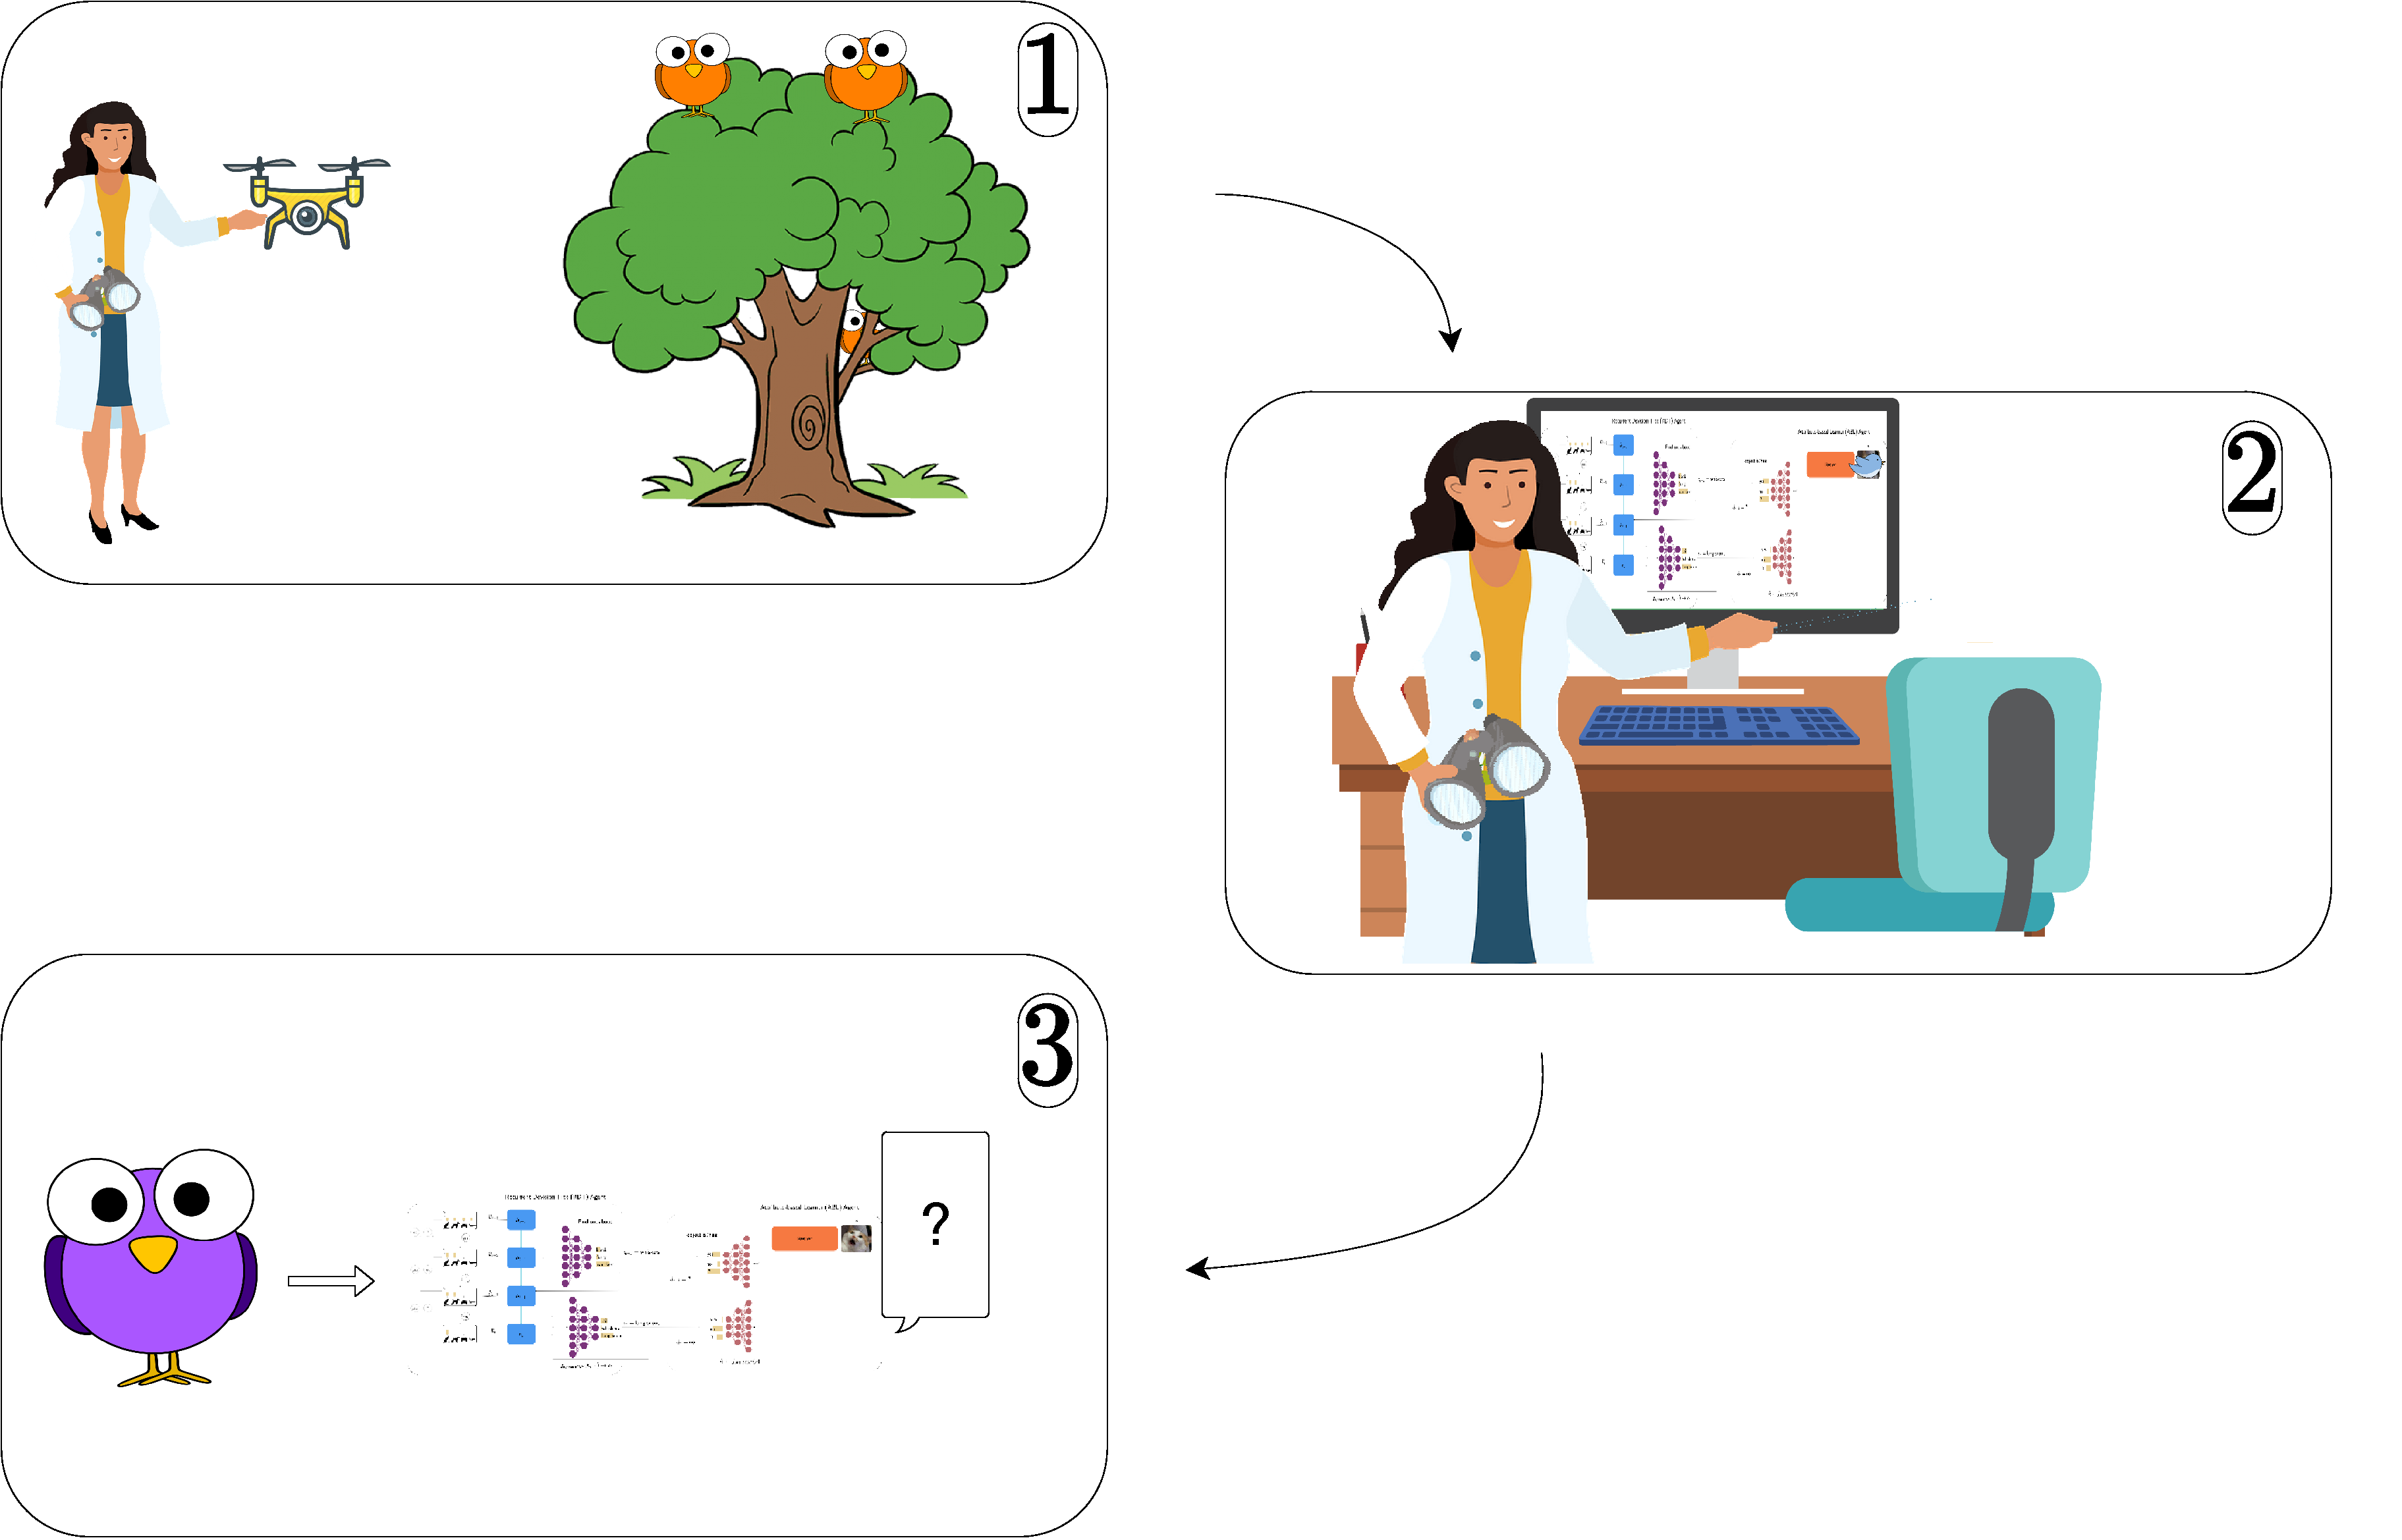
\includegraphics[width=0.9\textwidth]{ornithology.pdf}
	\caption{After collecting images of birds the ornithologist lets our proposed model classify the vast amount of data. Only in cases of high uncertainty, she is consulted and can classify the image manually.}
	\label{fig:qual}
\end{figure}

\section{Carbon Footprint Estimation}
% devices
To produce our results, we relied on GPUs provided by the University of Tübingen ML Cluster of Excellence and Google. We are aware of the profound impact, of the $CO_2$ emissions caused by producing the required electricity, on the world's climate.
The GPUs provided by Google were Nvidia Tesla K80 which operate up to the thermal design power of $300\;W$ \cite{nvidia2015tesla}. Devices of the University of Tübingen GPU cluster are Tesla V100-SXM2 which, at full capacity, operate up to a thermal design power of $300\;W$ \cite{nvidia2017tesla}. These specifications are without considering cooling.\\
% epochs
While no single model was trained for more than $50$ epochs, if we consider all models and all iterations of models, we accumulate about $2000$ epochs of training. Training time for one epoch was approximately $6$ minutes, or in $1$ hour, a model can be trained for $10$ epochs. Thus for $2000$ epochs, we get $200$ hours of training time. Considering the specification of our GPUs, we have consumed $200h * 300\;kW = 60000\;kWh$ of power.\\
% co equivalent
The German federal office for environmental concerns (Umweltbundesamt) estimates the amount of $CO_2$ necessary to produce one kilowatt-hour to be $401\;g$ \cite{icha2016entwicklung}. Considering, we required $60000\;kWh$, this would result in the $CO_2$ equivalent of $401\;g \cdot 60000 = 24060\;kg$.




\chapter{Conclusion}
Extending the work of \citet{alaniz2019explainable}, we propose an explainable model that is aware of and can express its uncertainties. The original model delivers a binary decision tree as an explanation, leveraging human-interpretable attributes, provided as side information. The nodes of the resulting tree correspond to attributes, and the edges to either 'Yes' or 'No' answers regarding the presence of these attributes. In our work, we give the model the ability to either avoid uncertain attributes to be used in the decision tree, or extend it to a ternary decision tree, where '?' is an additional option.\\
While our proposed extension does not outperform the original aRDTC model, our remRDTC and extRDTC still outperform other explainable methods such as decision trees or dNDF. Moreover, the performance is comparable to that of uninterpretable state of the art methods, such as ResNet.\\
Our model does not only utilize uncertainty information but also allows introspection. We use this to further investigate the relationship between attribute usage, misclassification and uncertainty.
We empirically show that our model (hopefully) reliable yields high uncertainty for unseen attributes. This would allow the model to consult a human user in cases of high uncertainty, thus making it more applicable in real-world scenarios.
Finally, we critically reflect the weaknesses of the model and propose possible improvements for future work.



\bibliographystyle{alpha}
\bibliography{bibliography}




\chapter*{Acknowledgments}
I would like to thank my pet snake, which sleeps all day, and my mother, who is the hardest working person I know. I would like to thank Zeynep and Stephan for the continuous support, their critical questions, and helpful insights.



\chapter*{Selbstst\"andigkeitserkl\"arung}
Hiermit versichere ich, dass ich die vorliegende Bachelorarbeit selbst\"andig und
nur mit den angegebenen Hilfsmitteln angefertigt habe und dass alle Stellen,
die dem Wortlaut oder dem Sinne nach anderen Werken entnommen sind,
durch Angaben von Quellen als Entlehnung kenntlich gemacht worden sind.
Diese Bachelorarbeit wurde in gleicher oder \"ahnlicher Form in keinem anderen
Studiengang als Pr\"ufungsleistung vorgelegt.

\vspace*{8ex}
\hrule
\vspace*{2ex}
Stefan Wezel (Matrikelnummer 4080589), \today

\end{document}

